\documentclass[twoside]{book}

% Packages required by doxygen
\usepackage{fixltx2e}
\usepackage{calc}
\usepackage{doxygen}
\usepackage[export]{adjustbox} % also loads graphicx
\usepackage{graphicx}
\usepackage[utf8]{inputenc}
\usepackage{makeidx}
\usepackage{multicol}
\usepackage{multirow}
\PassOptionsToPackage{warn}{textcomp}
\usepackage{textcomp}
\usepackage[nointegrals]{wasysym}
\usepackage[table]{xcolor}

% Font selection
\usepackage[T1]{fontenc}
\usepackage[scaled=.90]{helvet}
\usepackage{courier}
\usepackage{amssymb}
\usepackage{sectsty}
\renewcommand{\familydefault}{\sfdefault}
\allsectionsfont{%
  \fontseries{bc}\selectfont%
  \color{darkgray}%
}
\renewcommand{\DoxyLabelFont}{%
  \fontseries{bc}\selectfont%
  \color{darkgray}%
}
\newcommand{\+}{\discretionary{\mbox{\scriptsize$\hookleftarrow$}}{}{}}

% Page & text layout
\usepackage{geometry}
\geometry{%
  a4paper,%
  top=2.5cm,%
  bottom=2.5cm,%
  left=2.5cm,%
  right=2.5cm%
}
\tolerance=750
\hfuzz=15pt
\hbadness=750
\setlength{\emergencystretch}{15pt}
\setlength{\parindent}{0cm}
\setlength{\parskip}{3ex plus 2ex minus 2ex}
\makeatletter
\renewcommand{\paragraph}{%
  \@startsection{paragraph}{4}{0ex}{-1.0ex}{1.0ex}{%
    \normalfont\normalsize\bfseries\SS@parafont%
  }%
}
\renewcommand{\subparagraph}{%
  \@startsection{subparagraph}{5}{0ex}{-1.0ex}{1.0ex}{%
    \normalfont\normalsize\bfseries\SS@subparafont%
  }%
}
\makeatother

% Headers & footers
\usepackage{fancyhdr}
\pagestyle{fancyplain}
\fancyhead[LE]{\fancyplain{}{\bfseries\thepage}}
\fancyhead[CE]{\fancyplain{}{}}
\fancyhead[RE]{\fancyplain{}{\bfseries\leftmark}}
\fancyhead[LO]{\fancyplain{}{\bfseries\rightmark}}
\fancyhead[CO]{\fancyplain{}{}}
\fancyhead[RO]{\fancyplain{}{\bfseries\thepage}}
\fancyfoot[LE]{\fancyplain{}{}}
\fancyfoot[CE]{\fancyplain{}{}}
\fancyfoot[RE]{\fancyplain{}{\bfseries\scriptsize Generated by Doxygen }}
\fancyfoot[LO]{\fancyplain{}{\bfseries\scriptsize Generated by Doxygen }}
\fancyfoot[CO]{\fancyplain{}{}}
\fancyfoot[RO]{\fancyplain{}{}}
\renewcommand{\footrulewidth}{0.4pt}
\renewcommand{\chaptermark}[1]{%
  \markboth{#1}{}%
}
\renewcommand{\sectionmark}[1]{%
  \markright{\thesection\ #1}%
}

% Indices & bibliography
\usepackage{natbib}
\usepackage[titles]{tocloft}
\setcounter{tocdepth}{3}
\setcounter{secnumdepth}{5}
\makeindex

% Hyperlinks (required, but should be loaded last)
\usepackage{ifpdf}
\ifpdf
  \usepackage[pdftex,pagebackref=true]{hyperref}
\else
  \usepackage[ps2pdf,pagebackref=true]{hyperref}
\fi
\hypersetup{%
  colorlinks=true,%
  linkcolor=blue,%
  citecolor=blue,%
  unicode%
}

% Custom commands
\newcommand{\clearemptydoublepage}{%
  \newpage{\pagestyle{empty}\cleardoublepage}%
}

\usepackage{caption}
\captionsetup{labelsep=space,justification=centering,font={bf},singlelinecheck=off,skip=4pt,position=top}

%===== C O N T E N T S =====

\begin{document}

% Titlepage & ToC
\hypersetup{pageanchor=false,
             bookmarksnumbered=true,
             pdfencoding=unicode
            }
\pagenumbering{alph}
\begin{titlepage}
\vspace*{7cm}
\begin{center}%
{\Large My Project }\\
\vspace*{1cm}
{\large Generated by Doxygen 1.8.14}\\
\end{center}
\end{titlepage}
\clearemptydoublepage
\pagenumbering{roman}
\tableofcontents
\clearemptydoublepage
\pagenumbering{arabic}
\hypersetup{pageanchor=true}

%--- Begin generated contents ---
\chapter{Hierarchical Index}
\section{Class Hierarchy}
This inheritance list is sorted roughly, but not completely, alphabetically\+:\begin{DoxyCompactList}
\item \contentsline{section}{motion\+:\+:C\+Action\+Base}{\pageref{classmotion_1_1CActionBase}}{}
\begin{DoxyCompactList}
\item \contentsline{section}{motion\+:\+:C\+Action\+Arc}{\pageref{classmotion_1_1CActionArc}}{}
\item \contentsline{section}{motion\+:\+:C\+Action\+Backward}{\pageref{classmotion_1_1CActionBackward}}{}
\item \contentsline{section}{motion\+:\+:C\+Action\+Forward}{\pageref{classmotion_1_1CActionForward}}{}
\item \contentsline{section}{motion\+:\+:C\+Motion}{\pageref{classmotion_1_1CMotion}}{}
\item \contentsline{section}{motion\+:\+:C\+Motion\+Idle}{\pageref{classmotion_1_1CMotionIdle}}{}
\item \contentsline{section}{motion\+:\+:C\+Motion\+Point\+Tracker}{\pageref{classmotion_1_1CMotionPointTracker}}{}
\item \contentsline{section}{motion\+:\+:C\+Motion\+Wall\+Following}{\pageref{classmotion_1_1CMotionWallFollowing}}{}
\end{DoxyCompactList}
\item C\+My\+G\+L\+Canvas\+Base\begin{DoxyCompactList}
\item \contentsline{section}{C\+My\+G\+L\+Canvas}{\pageref{classCMyGLCanvas}}{}
\end{DoxyCompactList}
\item \contentsline{section}{motion\+:\+:C\+Path\+Generator}{\pageref{classmotion_1_1CPathGenerator}}{}
\item \contentsline{section}{motion\+:\+:C\+State$<$ state\+\_\+type $>$}{\pageref{classmotion_1_1CState}}{}
\item \contentsline{section}{motion\+:\+:C\+State$<$ C\+Motion $>$}{\pageref{classmotion_1_1CState}}{}
\begin{DoxyCompactList}
\item \contentsline{section}{motion\+:\+:C\+Motion\+Idle}{\pageref{classmotion_1_1CMotionIdle}}{}
\item \contentsline{section}{motion\+:\+:C\+Motion\+Point\+Tracker}{\pageref{classmotion_1_1CMotionPointTracker}}{}
\item \contentsline{section}{motion\+:\+:C\+Motion\+Wall\+Following}{\pageref{classmotion_1_1CMotionWallFollowing}}{}
\end{DoxyCompactList}
\item \contentsline{section}{motion\+:\+:C\+State$<$ C\+Motion\+Idle $>$}{\pageref{classmotion_1_1CState}}{}
\begin{DoxyCompactList}
\item \contentsline{section}{motion\+:\+:C\+Id\+Idle}{\pageref{classmotion_1_1CIdIdle}}{}
\end{DoxyCompactList}
\item \contentsline{section}{motion\+:\+:C\+State$<$ C\+Motion\+Point\+Tracker $>$}{\pageref{classmotion_1_1CState}}{}
\begin{DoxyCompactList}
\item \contentsline{section}{motion\+:\+:C\+P\+T\+Idle}{\pageref{classmotion_1_1CPTIdle}}{}
\item \contentsline{section}{motion\+:\+:C\+P\+T\+Tracking}{\pageref{classmotion_1_1CPTTracking}}{}
\end{DoxyCompactList}
\item \contentsline{section}{motion\+:\+:C\+State$<$ C\+Motion\+Wall\+Following $>$}{\pageref{classmotion_1_1CState}}{}
\begin{DoxyCompactList}
\item \contentsline{section}{motion\+:\+:C\+W\+F\+Obs\+Avoid}{\pageref{classmotion_1_1CWFObsAvoid}}{}
\item \contentsline{section}{motion\+:\+:C\+W\+F\+Ridge\+Track}{\pageref{classmotion_1_1CWFRidgeTrack}}{}
\item \contentsline{section}{motion\+:\+:C\+W\+F\+Wall\+Fol}{\pageref{classmotion_1_1CWFWallFol}}{}
\end{DoxyCompactList}
\item \contentsline{section}{motion\+:\+:C\+State$<$ motion\+:\+:C\+Motion $>$}{\pageref{classmotion_1_1CState}}{}
\item \contentsline{section}{motion\+:\+:C\+State$<$ motion\+:\+:C\+Motion\+Point\+Tracker $>$}{\pageref{classmotion_1_1CState}}{}
\item \contentsline{section}{motion\+:\+:C\+State$<$ motion\+:\+:C\+Motion\+Wall\+Following $>$}{\pageref{classmotion_1_1CState}}{}
\item \contentsline{section}{motion\+:\+:C\+State\+Machine$<$ state\+\_\+type $>$}{\pageref{classmotion_1_1CStateMachine}}{}
\item \contentsline{section}{motion\+:\+:C\+State\+Machine$<$ motion\+:\+:C\+Motion $>$}{\pageref{classmotion_1_1CStateMachine}}{}
\item \contentsline{section}{motion\+:\+:C\+State\+Machine$<$ motion\+:\+:C\+Motion\+Point\+Tracker $>$}{\pageref{classmotion_1_1CStateMachine}}{}
\item \contentsline{section}{motion\+:\+:C\+State\+Machine$<$ motion\+:\+:C\+Motion\+Wall\+Following $>$}{\pageref{classmotion_1_1CStateMachine}}{}
\item \contentsline{section}{motion\+:\+:T\+Motion}{\pageref{structmotion_1_1TMotion}}{}
\item \contentsline{section}{motion\+:\+:T\+Motion\+Params}{\pageref{structmotion_1_1TMotionParams}}{}
\item \contentsline{section}{T\+Motion\+P\+I\+D\+Con}{\pageref{structTMotionPIDCon}}{}
\item \contentsline{section}{motion\+:\+:T\+Motion\+Point}{\pageref{structmotion_1_1TMotionPoint}}{}
\item \contentsline{section}{motion\+:\+:T\+Motion\+Pose2D}{\pageref{structmotion_1_1TMotionPose2D}}{}
\item \contentsline{section}{motion\+:\+:T\+Motion\+Vector2D}{\pageref{structmotion_1_1TMotionVector2D}}{}
\item \contentsline{section}{Vector2D}{\pageref{structVector2D}}{}
\item wx\+App\begin{DoxyCompactList}
\item \contentsline{section}{gridmap\+Simul\+App}{\pageref{classgridmapSimulApp}}{}
\end{DoxyCompactList}
\item wx\+Art\+Provider\begin{DoxyCompactList}
\item \contentsline{section}{My\+Art\+Provider}{\pageref{classMyArtProvider}}{}
\end{DoxyCompactList}
\item wx\+Dialog\begin{DoxyCompactList}
\item \contentsline{section}{C\+About\+Box}{\pageref{classCAboutBox}}{}
\end{DoxyCompactList}
\item wx\+Frame\begin{DoxyCompactList}
\item \contentsline{section}{gridmap\+Simul\+Frame}{\pageref{classgridmapSimulFrame}}{}
\end{DoxyCompactList}
\end{DoxyCompactList}

\chapter{Class Index}
\section{Class List}
Here are the classes, structs, unions and interfaces with brief descriptions\+:\begin{DoxyCompactList}
\item\contentsline{section}{\mbox{\hyperlink{classCAboutBox}{C\+About\+Box}} }{\pageref{classCAboutBox}}{}
\item\contentsline{section}{\mbox{\hyperlink{classmotion_1_1CActionArc}{motion\+::\+C\+Action\+Arc}} }{\pageref{classmotion_1_1CActionArc}}{}
\item\contentsline{section}{\mbox{\hyperlink{classmotion_1_1CActionBackward}{motion\+::\+C\+Action\+Backward}} }{\pageref{classmotion_1_1CActionBackward}}{}
\item\contentsline{section}{\mbox{\hyperlink{classmotion_1_1CActionBase}{motion\+::\+C\+Action\+Base}} }{\pageref{classmotion_1_1CActionBase}}{}
\item\contentsline{section}{\mbox{\hyperlink{classmotion_1_1CActionForward}{motion\+::\+C\+Action\+Forward}} }{\pageref{classmotion_1_1CActionForward}}{}
\item\contentsline{section}{\mbox{\hyperlink{classmotion_1_1CMotionWallFollowing}{motion\+::\+C\+Motion\+Wall\+Following}} }{\pageref{classmotion_1_1CMotionWallFollowing}}{}
\item\contentsline{section}{\mbox{\hyperlink{classCMyGLCanvas}{C\+My\+G\+L\+Canvas}} }{\pageref{classCMyGLCanvas}}{}
\item\contentsline{section}{\mbox{\hyperlink{classmotion_1_1CState}{motion\+::\+C\+State$<$ state\+\_\+type $>$}} }{\pageref{classmotion_1_1CState}}{}
\item\contentsline{section}{\mbox{\hyperlink{classmotion_1_1CStateMachine}{motion\+::\+C\+State\+Machine$<$ state\+\_\+type $>$}} }{\pageref{classmotion_1_1CStateMachine}}{}
\item\contentsline{section}{\mbox{\hyperlink{classgridmapSimulApp}{gridmap\+Simul\+App}} }{\pageref{classgridmapSimulApp}}{}
\item\contentsline{section}{\mbox{\hyperlink{classgridmapSimulFrame}{gridmap\+Simul\+Frame}} }{\pageref{classgridmapSimulFrame}}{}
\item\contentsline{section}{\mbox{\hyperlink{classMyArtProvider}{My\+Art\+Provider}} }{\pageref{classMyArtProvider}}{}
\item\contentsline{section}{\mbox{\hyperlink{structmotion_1_1TMotionPose2D}{motion\+::\+T\+Motion\+Pose2D}} }{\pageref{structmotion_1_1TMotionPose2D}}{}
\item\contentsline{section}{\mbox{\hyperlink{structVector2D}{Vector2D}} }{\pageref{structVector2D}}{}
\end{DoxyCompactList}

\chapter{Class Documentation}
\hypertarget{classCAboutBox}{}\section{C\+About\+Box Class Reference}
\label{classCAboutBox}\index{C\+About\+Box@{C\+About\+Box}}
Inheritance diagram for C\+About\+Box\+:\begin{figure}[H]
\begin{center}
\leavevmode
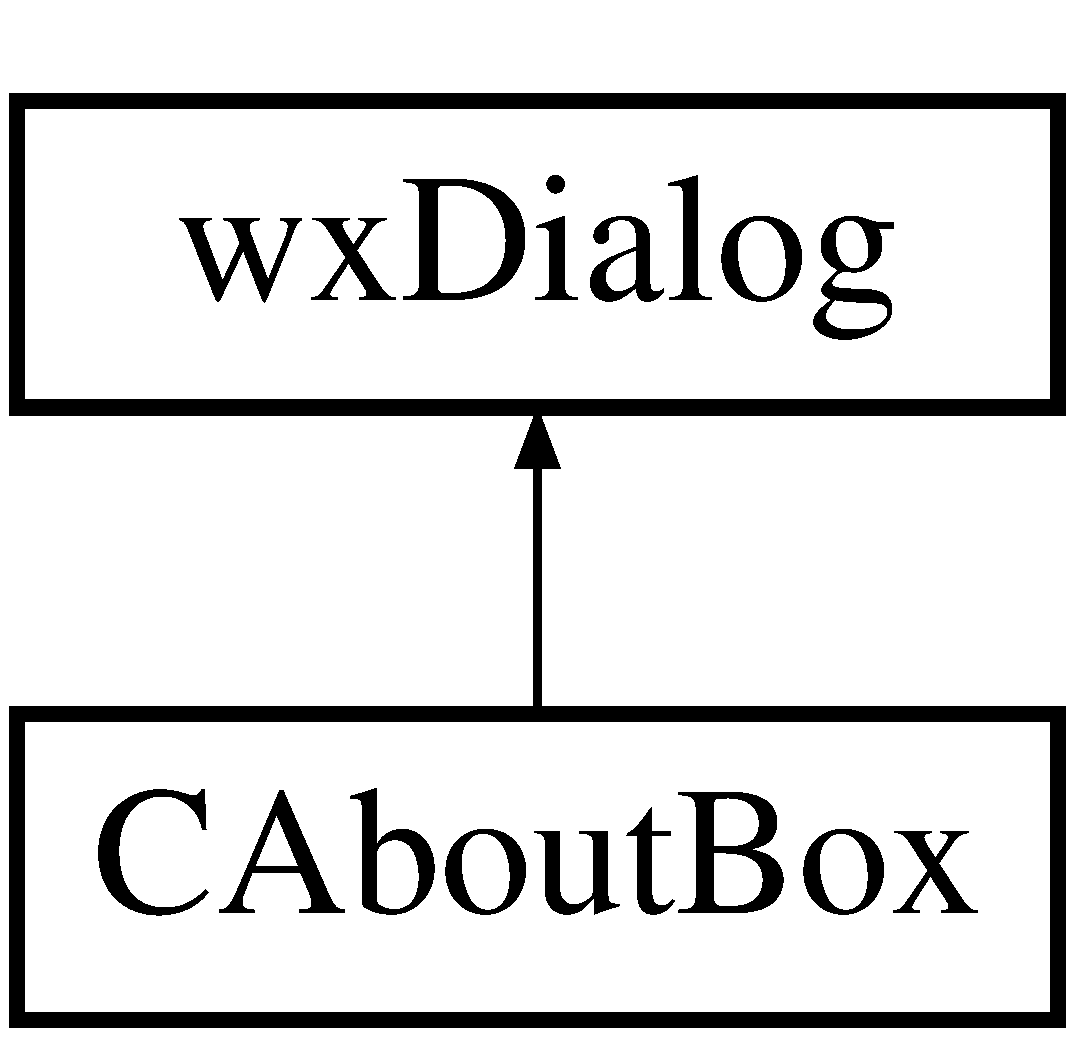
\includegraphics[height=2.000000cm]{classCAboutBox}
\end{center}
\end{figure}
\subsection*{Public Member Functions}
\begin{DoxyCompactItemize}
\item 
\mbox{\Hypertarget{classCAboutBox_ac23aeafcffb40eb72b01da54b7db8e37}\label{classCAboutBox_ac23aeafcffb40eb72b01da54b7db8e37}} 
{\bfseries C\+About\+Box} (wx\+Window $\ast$parent, wx\+Window\+ID id=-\/1)
\end{DoxyCompactItemize}
\subsection*{Static Public Attributes}
\begin{DoxyCompactItemize}
\item 
\mbox{\Hypertarget{classCAboutBox_a8a8c71cf80bae706d4dcab85ea36330f}\label{classCAboutBox_a8a8c71cf80bae706d4dcab85ea36330f}} 
static const long {\bfseries I\+D\+\_\+\+S\+T\+A\+T\+I\+C\+T\+E\+X\+T1} = wx\+New\+Id()
\item 
\mbox{\Hypertarget{classCAboutBox_ad9232b25d16dc3fd4118b66356de9835}\label{classCAboutBox_ad9232b25d16dc3fd4118b66356de9835}} 
static const long {\bfseries I\+D\+\_\+\+S\+T\+A\+T\+I\+C\+T\+E\+X\+T2} = wx\+New\+Id()
\item 
\mbox{\Hypertarget{classCAboutBox_a0a488920494fd9877808ab6161460f50}\label{classCAboutBox_a0a488920494fd9877808ab6161460f50}} 
static const long {\bfseries I\+D\+\_\+\+S\+T\+A\+T\+I\+C\+B\+I\+T\+M\+A\+P1} = wx\+New\+Id()
\item 
\mbox{\Hypertarget{classCAboutBox_a37f53de8b8107dd06c492ede246d1666}\label{classCAboutBox_a37f53de8b8107dd06c492ede246d1666}} 
static const long {\bfseries I\+D\+\_\+\+S\+T\+A\+T\+I\+C\+L\+I\+N\+E1} = wx\+New\+Id()
\item 
\mbox{\Hypertarget{classCAboutBox_a0d649c670b29575cdbfc1f1a1a6ad177}\label{classCAboutBox_a0d649c670b29575cdbfc1f1a1a6ad177}} 
static const long {\bfseries I\+D\+\_\+\+T\+E\+X\+T\+C\+T\+R\+L1} = wx\+New\+Id()
\item 
\mbox{\Hypertarget{classCAboutBox_a6c8d3fabb2794f7bacfcf641aaf23abb}\label{classCAboutBox_a6c8d3fabb2794f7bacfcf641aaf23abb}} 
static const long {\bfseries I\+D\+\_\+\+T\+E\+X\+T\+C\+T\+R\+L2} = wx\+New\+Id()
\item 
\mbox{\Hypertarget{classCAboutBox_ab111166245ba1ed7e7a51820faf25aa3}\label{classCAboutBox_ab111166245ba1ed7e7a51820faf25aa3}} 
static const long {\bfseries I\+D\+\_\+\+T\+E\+X\+T\+C\+T\+R\+L3} = wx\+New\+Id()
\item 
\mbox{\Hypertarget{classCAboutBox_a1b9b6bcf1535e4ba4a6f122d59c74f20}\label{classCAboutBox_a1b9b6bcf1535e4ba4a6f122d59c74f20}} 
static const long {\bfseries I\+D\+\_\+\+N\+O\+T\+E\+B\+O\+O\+K1} = wx\+New\+Id()
\item 
\mbox{\Hypertarget{classCAboutBox_a709e9b214b7b73ecd7f194d1212ba872}\label{classCAboutBox_a709e9b214b7b73ecd7f194d1212ba872}} 
static const long {\bfseries I\+D\+\_\+\+B\+U\+T\+T\+O\+N1} = wx\+New\+Id()
\end{DoxyCompactItemize}
\subsection*{Protected Member Functions}
\begin{DoxyCompactItemize}
\item 
\mbox{\Hypertarget{classCAboutBox_a7b8a029f1bc14a171489139ecf3b9efd}\label{classCAboutBox_a7b8a029f1bc14a171489139ecf3b9efd}} 
void {\bfseries On\+Init} (wx\+Init\+Dialog\+Event \&event)
\item 
\mbox{\Hypertarget{classCAboutBox_a4ceb56a1d2dcdf7ebdbc2db415abcf00}\label{classCAboutBox_a4ceb56a1d2dcdf7ebdbc2db415abcf00}} 
void {\bfseries On\+Button1\+Click} (wx\+Command\+Event \&event)
\item 
\mbox{\Hypertarget{classCAboutBox_a8ba8776862019cee447e0cce4cfa58df}\label{classCAboutBox_a8ba8776862019cee447e0cce4cfa58df}} 
void {\bfseries On\+Char} (wx\+Key\+Event \&event)
\end{DoxyCompactItemize}
\subsection*{Protected Attributes}
\begin{DoxyCompactItemize}
\item 
\mbox{\Hypertarget{classCAboutBox_a0250ce66d89cd0c47107d23d7823b550}\label{classCAboutBox_a0250ce66d89cd0c47107d23d7823b550}} 
wx\+Static\+Text $\ast$ {\bfseries lb\+Prog\+Name}
\item 
\mbox{\Hypertarget{classCAboutBox_a7eb4127fb53f0df92c73ced7c9d8704b}\label{classCAboutBox_a7eb4127fb53f0df92c73ced7c9d8704b}} 
wx\+Flex\+Grid\+Sizer $\ast$ {\bfseries Flex\+Grid\+Sizer1}
\item 
\mbox{\Hypertarget{classCAboutBox_af39fc1e955543ca8e4dc60d900e29339}\label{classCAboutBox_af39fc1e955543ca8e4dc60d900e29339}} 
wx\+Text\+Ctrl $\ast$ {\bfseries lb\+License}
\item 
\mbox{\Hypertarget{classCAboutBox_a6ee2c45e8140523726ae0adac39e5e8d}\label{classCAboutBox_a6ee2c45e8140523726ae0adac39e5e8d}} 
wx\+Button $\ast$ {\bfseries Button1}
\item 
\mbox{\Hypertarget{classCAboutBox_a03cbdcae864388315c72bc1b301cc079}\label{classCAboutBox_a03cbdcae864388315c72bc1b301cc079}} 
wx\+Flex\+Grid\+Sizer $\ast$ {\bfseries Flex\+Grid\+Sizer4}
\item 
\mbox{\Hypertarget{classCAboutBox_a3839eefb2b7f455608fd9e84893fd404}\label{classCAboutBox_a3839eefb2b7f455608fd9e84893fd404}} 
wx\+Static\+Line $\ast$ {\bfseries Static\+Line1}
\item 
\mbox{\Hypertarget{classCAboutBox_ac2602c693f6375acace0ffc56f3a62c5}\label{classCAboutBox_ac2602c693f6375acace0ffc56f3a62c5}} 
wx\+Static\+Text $\ast$ {\bfseries lb\+Build}
\item 
\mbox{\Hypertarget{classCAboutBox_a1b4ced1fdb78e6579f120a14aa1db7ec}\label{classCAboutBox_a1b4ced1fdb78e6579f120a14aa1db7ec}} 
wx\+Text\+Ctrl $\ast$ {\bfseries Text\+Ctrl1}
\item 
\mbox{\Hypertarget{classCAboutBox_a34c7e54c89dca93bdc268582e9b135c4}\label{classCAboutBox_a34c7e54c89dca93bdc268582e9b135c4}} 
wx\+Notebook $\ast$ {\bfseries Notebook1}
\item 
\mbox{\Hypertarget{classCAboutBox_ab8d715f8ada37310f3d43b81b739f979}\label{classCAboutBox_ab8d715f8ada37310f3d43b81b739f979}} 
wx\+Text\+Ctrl $\ast$ {\bfseries lb\+Info}
\item 
\mbox{\Hypertarget{classCAboutBox_ad691d2c2a7dd5252942841d72883ccdd}\label{classCAboutBox_ad691d2c2a7dd5252942841d72883ccdd}} 
wx\+Static\+Bitmap $\ast$ {\bfseries Static\+Bitmap1}
\end{DoxyCompactItemize}


The documentation for this class was generated from the following files\+:\begin{DoxyCompactItemize}
\item 
C\+About\+Box.\+h\item 
C\+About\+Box.\+cpp\end{DoxyCompactItemize}

\hypertarget{classmotion_1_1CActionArc}{}\section{motion\+:\+:C\+Action\+Arc Class Reference}
\label{classmotion_1_1CActionArc}\index{motion\+::\+C\+Action\+Arc@{motion\+::\+C\+Action\+Arc}}
Inheritance diagram for motion\+:\+:C\+Action\+Arc\+:\begin{figure}[H]
\begin{center}
\leavevmode
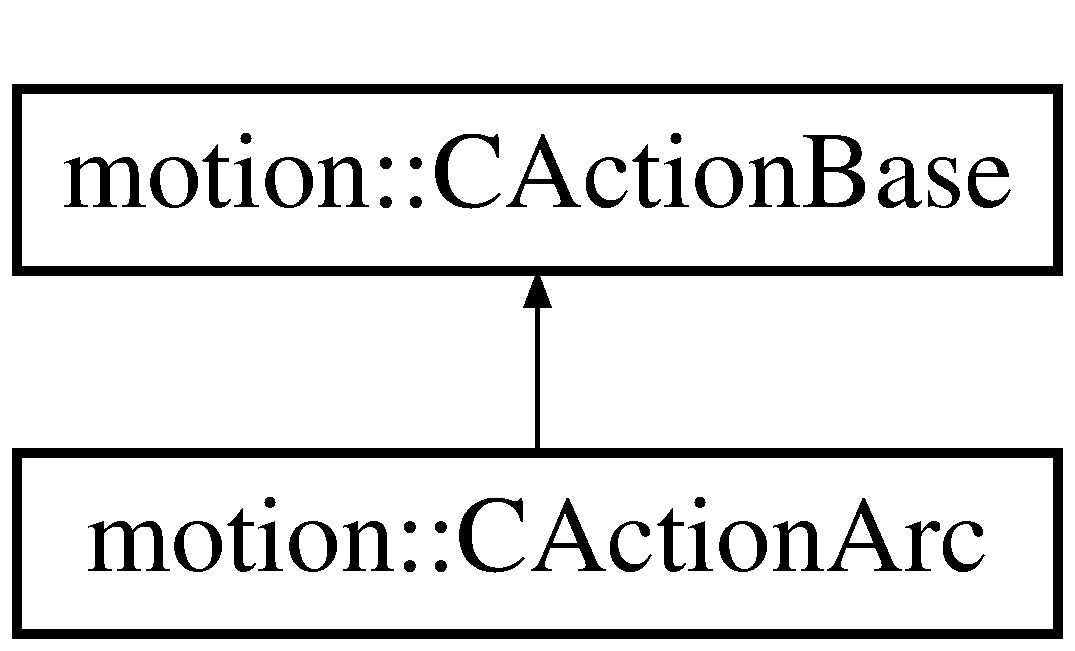
\includegraphics[height=2.000000cm]{classmotion_1_1CActionArc}
\end{center}
\end{figure}
\subsection*{Public Member Functions}
\begin{DoxyCompactItemize}
\item 
\mbox{\Hypertarget{classmotion_1_1CActionArc_a7b8746c8652bb865f2b606608dffbb16}\label{classmotion_1_1CActionArc_a7b8746c8652bb865f2b606608dffbb16}} 
void {\bfseries reset} (void)
\item 
\mbox{\Hypertarget{classmotion_1_1CActionArc_a45356c022471267db143fd1300f6b465}\label{classmotion_1_1CActionArc_a45356c022471267db143fd1300f6b465}} 
void {\bfseries set\+State} (E\+Steering\+State\+Type state)
\item 
\mbox{\Hypertarget{classmotion_1_1CActionArc_ad6f08adc549f8d19892e0a6a257415dc}\label{classmotion_1_1CActionArc_ad6f08adc549f8d19892e0a6a257415dc}} 
void {\bfseries set\+End\+Pose} (\mbox{\hyperlink{structmotion_1_1TMotionPose2D}{T\+Motion\+Pose2D}} pose)
\item 
\mbox{\Hypertarget{classmotion_1_1CActionArc_a6af47c85b3b8226b6ae5bc3e27185e77}\label{classmotion_1_1CActionArc_a6af47c85b3b8226b6ae5bc3e27185e77}} 
void {\bfseries set\+Start\+Up} (bool val)
\item 
\mbox{\Hypertarget{classmotion_1_1CActionArc_ae196348547fee7f670bb91f66b55fa36}\label{classmotion_1_1CActionArc_ae196348547fee7f670bb91f66b55fa36}} 
E\+Steering\+State\+Type {\bfseries get\+State} (void)
\item 
\mbox{\Hypertarget{classmotion_1_1CActionArc_ad5ff8628c709a14cbcffb030894daa93}\label{classmotion_1_1CActionArc_ad5ff8628c709a14cbcffb030894daa93}} 
\mbox{\hyperlink{structmotion_1_1TMotionPose2D}{T\+Motion\+Pose2D}} {\bfseries get\+End\+Pose} (void)
\item 
\mbox{\Hypertarget{classmotion_1_1CActionArc_aa2ee90e89b02256cd0c3f422f220caca}\label{classmotion_1_1CActionArc_aa2ee90e89b02256cd0c3f422f220caca}} 
bool {\bfseries get\+Start\+Up} (void)
\item 
void \mbox{\hyperlink{classmotion_1_1CActionArc_a64a6fc339df29d196786291f02b2802e}{arc}} (double w, double ang\+Deg, double radius=0)
\end{DoxyCompactItemize}
\subsection*{Static Public Member Functions}
\begin{DoxyCompactItemize}
\item 
\mbox{\Hypertarget{classmotion_1_1CActionArc_a058d43888af190cf93dc3130746d9e9e}\label{classmotion_1_1CActionArc_a058d43888af190cf93dc3130746d9e9e}} 
static \mbox{\hyperlink{classmotion_1_1CActionArc}{C\+Action\+Arc}} $\ast$ {\bfseries get\+Instance} (void)
\end{DoxyCompactItemize}


\subsection{Member Function Documentation}
\mbox{\Hypertarget{classmotion_1_1CActionArc_a64a6fc339df29d196786291f02b2802e}\label{classmotion_1_1CActionArc_a64a6fc339df29d196786291f02b2802e}} 
\index{motion\+::\+C\+Action\+Arc@{motion\+::\+C\+Action\+Arc}!arc@{arc}}
\index{arc@{arc}!motion\+::\+C\+Action\+Arc@{motion\+::\+C\+Action\+Arc}}
\subsubsection{\texorpdfstring{arc()}{arc()}}
{\footnotesize\ttfamily void C\+Action\+Arc\+::arc (\begin{DoxyParamCaption}\item[{double}]{w,  }\item[{double}]{ang\+Deg,  }\item[{double}]{radius = {\ttfamily 0} }\end{DoxyParamCaption})}

Make the vehicle make arc. 
\begin{DoxyParams}{Parameters}
{\em w} & Linear velocity(rad/s). w is positive. \\
\hline
{\em angle\+Degree} & The desired angle in degree we want the robot rotate. angle\+Degree $>$ 0 rotate counterclockwise. \\
\hline
{\em radius} & Arc radius. \\
\hline
\end{DoxyParams}
how to avoid multiple tasks? ~\newline
~\newline
~\newline
~\newline
 Start the timer

If start up is enabled, update if the vehicle get started everytime. ~\newline
~\newline
 throw exceptions assert(!\char`\"{}\+Time out when making Arc move.\char`\"{}); ~\newline
 throw exceptions assert(!\char`\"{}\+Direction reached but can\textquotesingle{}t reach the appropriate location.\char`\"{}); 

The documentation for this class was generated from the following files\+:\begin{DoxyCompactItemize}
\item 
motion/action/C\+Action\+Arc.\+h\item 
motion/action/C\+Action\+Arc.\+cpp\end{DoxyCompactItemize}

\hypertarget{classmotion_1_1CActionBackward}{}\section{motion\+:\+:C\+Action\+Backward Class Reference}
\label{classmotion_1_1CActionBackward}\index{motion\+::\+C\+Action\+Backward@{motion\+::\+C\+Action\+Backward}}


{\ttfamily \#include $<$C\+Action\+Backward.\+h$>$}

Inheritance diagram for motion\+:\+:C\+Action\+Backward\+:\begin{figure}[H]
\begin{center}
\leavevmode
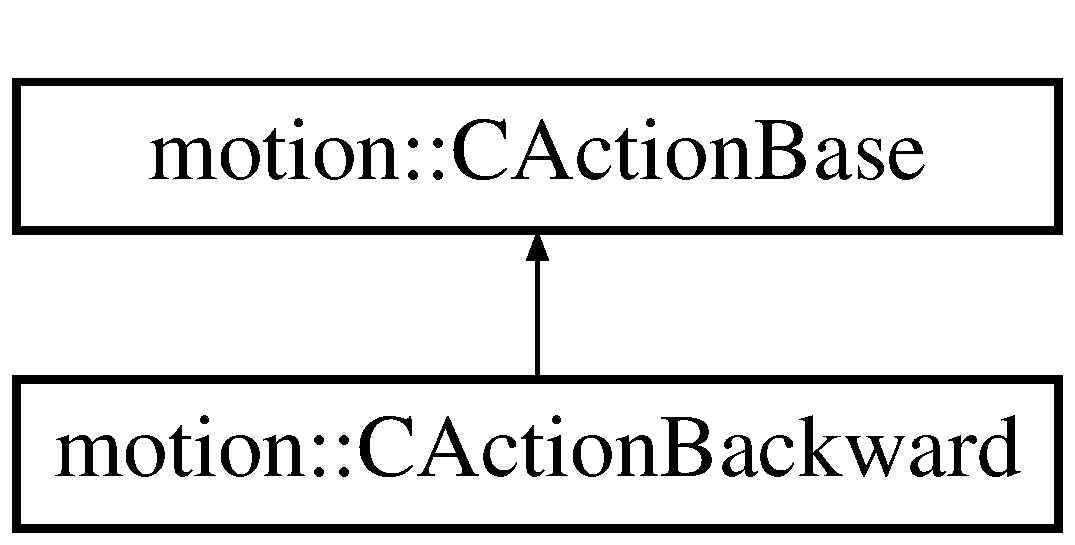
\includegraphics[height=2.000000cm]{classmotion_1_1CActionBackward}
\end{center}
\end{figure}
\subsection*{Public Member Functions}
\begin{DoxyCompactItemize}
\item 
void \mbox{\hyperlink{classmotion_1_1CActionBackward_a609f364c24b4ceebda81c0b591692d2a}{reset}} (void)
\item 
void \mbox{\hyperlink{classmotion_1_1CActionBackward_ab05c93abef4815a4a9f38afeddbb8c2a}{backward}} (double v, double distance)
\end{DoxyCompactItemize}
\subsection*{Static Public Member Functions}
\begin{DoxyCompactItemize}
\item 
\mbox{\Hypertarget{classmotion_1_1CActionBackward_aa1b0a2ac1a8f390bc88b36607137b5f1}\label{classmotion_1_1CActionBackward_aa1b0a2ac1a8f390bc88b36607137b5f1}} 
static \mbox{\hyperlink{classmotion_1_1CActionBackward}{C\+Action\+Backward}} $\ast$ {\bfseries get\+Instance} (void)
\end{DoxyCompactItemize}


\subsection{Detailed Description}
Backward ~\newline
 example\+: ~\newline
 \#include \mbox{\hyperlink{CActionBackward_8h}{C\+Action\+Backward.\+h}} ~\newline
 bkw-\/$>$backward(1, 90); ~\newline
if(bkw-\/$>$get\+Action\+State()==B\+A\+C\+K\+W\+A\+R\+D\+\_\+\+F\+I\+N\+I\+S\+H\+ED) ~\newline
\{ ~\newline
 printf(\char`\"{}\+Backing task finished. Please command the next order.\textbackslash{}n\char`\"{}); ~\newline
\} 

\subsection{Member Function Documentation}
\mbox{\Hypertarget{classmotion_1_1CActionBackward_ab05c93abef4815a4a9f38afeddbb8c2a}\label{classmotion_1_1CActionBackward_ab05c93abef4815a4a9f38afeddbb8c2a}} 
\index{motion\+::\+C\+Action\+Backward@{motion\+::\+C\+Action\+Backward}!backward@{backward}}
\index{backward@{backward}!motion\+::\+C\+Action\+Backward@{motion\+::\+C\+Action\+Backward}}
\subsubsection{\texorpdfstring{backward()}{backward()}}
{\footnotesize\ttfamily void C\+Action\+Backward\+::backward (\begin{DoxyParamCaption}\item[{double}]{v,  }\item[{double}]{distance }\end{DoxyParamCaption})}

Move the robot backward straightly. 
\begin{DoxyParams}{Parameters}
{\em v} & The backward linear velocity. \\
\hline
{\em distance} & The desired distance we want the robot backward. \\
\hline
\end{DoxyParams}
Store current information and calculate information needed

start the timer

Timeout check.

throw exceptions assert(!\char`\"{}\+Time out when backwarding.\char`\"{}); ~\newline
 Finish condition check. \mbox{\Hypertarget{classmotion_1_1CActionBackward_a609f364c24b4ceebda81c0b591692d2a}\label{classmotion_1_1CActionBackward_a609f364c24b4ceebda81c0b591692d2a}} 
\index{motion\+::\+C\+Action\+Backward@{motion\+::\+C\+Action\+Backward}!reset@{reset}}
\index{reset@{reset}!motion\+::\+C\+Action\+Backward@{motion\+::\+C\+Action\+Backward}}
\subsubsection{\texorpdfstring{reset()}{reset()}}
{\footnotesize\ttfamily void C\+Action\+Backward\+::reset (\begin{DoxyParamCaption}\item[{void}]{ }\end{DoxyParamCaption})}

$<$ Reset base private variables. 

The documentation for this class was generated from the following files\+:\begin{DoxyCompactItemize}
\item 
motion/action/\mbox{\hyperlink{CActionBackward_8h}{C\+Action\+Backward.\+h}}\item 
motion/action/\mbox{\hyperlink{CActionBackward_8cpp}{C\+Action\+Backward.\+cpp}}\end{DoxyCompactItemize}

\hypertarget{classmotion_1_1CActionBase}{}\section{motion\+:\+:C\+Action\+Base Class Reference}
\label{classmotion_1_1CActionBase}\index{motion\+::\+C\+Action\+Base@{motion\+::\+C\+Action\+Base}}


{\ttfamily \#include $<$C\+Action\+Base.\+h$>$}

Inheritance diagram for motion\+:\+:C\+Action\+Base\+:\begin{figure}[H]
\begin{center}
\leavevmode
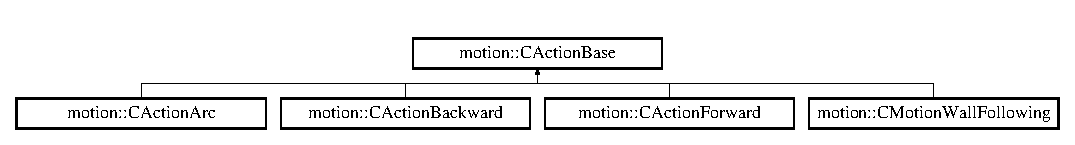
\includegraphics[height=0.855615cm]{classmotion_1_1CActionBase}
\end{center}
\end{figure}
\subsection*{Public Member Functions}
\begin{DoxyCompactItemize}
\item 
\mbox{\Hypertarget{classmotion_1_1CActionBase_ab64789ff634b40a7c88771186deb02b3}\label{classmotion_1_1CActionBase_ab64789ff634b40a7c88771186deb02b3}} 
void {\bfseries reset\+Base} (void)
\item 
\mbox{\Hypertarget{classmotion_1_1CActionBase_a56290a85c15b62718137f4a79a0e5d24}\label{classmotion_1_1CActionBase_a56290a85c15b62718137f4a79a0e5d24}} 
double {\bfseries get\+Ahead\+Dist} (void) const
\item 
\mbox{\Hypertarget{classmotion_1_1CActionBase_adee7bb394fc82f936af57e997ccc1f7f}\label{classmotion_1_1CActionBase_adee7bb394fc82f936af57e997ccc1f7f}} 
double {\bfseries get\+Side\+Dist} (void) const
\item 
\mbox{\Hypertarget{classmotion_1_1CActionBase_ab7cac53d714c3688609f5bfb026c6c4f}\label{classmotion_1_1CActionBase_ab7cac53d714c3688609f5bfb026c6c4f}} 
double {\bfseries get\+Linear\+Velocity} (void) const
\item 
\mbox{\Hypertarget{classmotion_1_1CActionBase_aba9b4953364ac77f49e98ea6f59a3aad}\label{classmotion_1_1CActionBase_aba9b4953364ac77f49e98ea6f59a3aad}} 
void {\bfseries set\+Velocity} (double v, double w)
\item 
\mbox{\Hypertarget{classmotion_1_1CActionBase_ab83e2ccbad3a796da9c8013467f89a5d}\label{classmotion_1_1CActionBase_ab83e2ccbad3a796da9c8013467f89a5d}} 
void {\bfseries set\+Motion} (\mbox{\hyperlink{motionEnums_8h_a907f80786f402332d43f4646dc1450bc}{E\+Motion}} mot)
\item 
\mbox{\Hypertarget{classmotion_1_1CActionBase_a97b30f5e328649e00b8c3889ef6fce4a}\label{classmotion_1_1CActionBase_a97b30f5e328649e00b8c3889ef6fce4a}} 
void {\bfseries set\+Sub\+Motion} (\mbox{\hyperlink{motionEnums_8h_a23be5ef75af9219a8bf688fd9716d72c}{E\+Sub\+Motion}} submot)
\item 
\mbox{\Hypertarget{classmotion_1_1CActionBase_a82ea8bab8f8a6ccfe0f4cf4addc47d33}\label{classmotion_1_1CActionBase_a82ea8bab8f8a6ccfe0f4cf4addc47d33}} 
void {\bfseries set\+Sub\+Motion\+State} (\mbox{\hyperlink{motionEnums_8h_a272f94c6143b9acf7ac44f165be53948}{E\+Sub\+Motion\+State}} submotstate)
\item 
\mbox{\Hypertarget{classmotion_1_1CActionBase_aa5ea8ef039688efb9da75e552bfff955}\label{classmotion_1_1CActionBase_aa5ea8ef039688efb9da75e552bfff955}} 
void {\bfseries set\+Action} (\mbox{\hyperlink{motionEnums_8h_aa7486027d362655230b958efe6985a7f}{E\+Action}} act) const
\item 
\mbox{\Hypertarget{classmotion_1_1CActionBase_a37cf7cf8e21e5df22d1ae5326e92db63}\label{classmotion_1_1CActionBase_a37cf7cf8e21e5df22d1ae5326e92db63}} 
void {\bfseries set\+Action\+State} (\mbox{\hyperlink{motionEnums_8h_ac80e838bea11b75469bfc14b1de921a3}{E\+Action\+State}} actsta)
\item 
\mbox{\Hypertarget{classmotion_1_1CActionBase_a9c30abb08480e7b0cbd8a2d1bd2289a9}\label{classmotion_1_1CActionBase_a9c30abb08480e7b0cbd8a2d1bd2289a9}} 
\mbox{\hyperlink{motionEnums_8h_a907f80786f402332d43f4646dc1450bc}{E\+Motion}} {\bfseries get\+Motion} (void) const
\item 
\mbox{\Hypertarget{classmotion_1_1CActionBase_ade6e14ed3cdb446bc146c4188d845547}\label{classmotion_1_1CActionBase_ade6e14ed3cdb446bc146c4188d845547}} 
\mbox{\hyperlink{motionEnums_8h_a23be5ef75af9219a8bf688fd9716d72c}{E\+Sub\+Motion}} {\bfseries get\+Sub\+Motion} (void) const
\item 
\mbox{\Hypertarget{classmotion_1_1CActionBase_a51e0207c21bc6da29b0435dead1dd6cc}\label{classmotion_1_1CActionBase_a51e0207c21bc6da29b0435dead1dd6cc}} 
\mbox{\hyperlink{motionEnums_8h_a272f94c6143b9acf7ac44f165be53948}{E\+Sub\+Motion\+State}} {\bfseries get\+Sub\+Motion\+State} (void) const
\item 
\mbox{\Hypertarget{classmotion_1_1CActionBase_a14d5ba8c773b1abb71974777daa5e0da}\label{classmotion_1_1CActionBase_a14d5ba8c773b1abb71974777daa5e0da}} 
\mbox{\hyperlink{motionEnums_8h_aa7486027d362655230b958efe6985a7f}{E\+Action}} {\bfseries get\+Action} (void) const
\item 
\mbox{\Hypertarget{classmotion_1_1CActionBase_af0210e352a49c47ad7a7a2d2d8145a63}\label{classmotion_1_1CActionBase_af0210e352a49c47ad7a7a2d2d8145a63}} 
\mbox{\hyperlink{motionEnums_8h_ac80e838bea11b75469bfc14b1de921a3}{E\+Action\+State}} {\bfseries get\+Action\+State} (void) const
\item 
\mbox{\Hypertarget{classmotion_1_1CActionBase_a6c91610ed7b320cfc5ed13cfea9494b5}\label{classmotion_1_1CActionBase_a6c91610ed7b320cfc5ed13cfea9494b5}} 
double {\bfseries get\+Angular\+Velocity} (void)
\item 
\mbox{\Hypertarget{classmotion_1_1CActionBase_a7fcc833fc87392ea9f8990217c699990}\label{classmotion_1_1CActionBase_a7fcc833fc87392ea9f8990217c699990}} 
bool {\bfseries get\+Pose\+Stored} (void) const
\item 
\mbox{\Hypertarget{classmotion_1_1CActionBase_a1e4ce35712fb80d112e93f4c0025a17a}\label{classmotion_1_1CActionBase_a1e4ce35712fb80d112e93f4c0025a17a}} 
void {\bfseries set\+Pose\+Stored} (bool flag)
\item 
\mbox{\Hypertarget{classmotion_1_1CActionBase_ac576f7b9fffaa9b682b78e3737d73e36}\label{classmotion_1_1CActionBase_ac576f7b9fffaa9b682b78e3737d73e36}} 
\mbox{\hyperlink{structmotion_1_1TMotionPose2D}{T\+Motion\+Pose2D}} {\bfseries get\+Start\+Pose} (void) const
\item 
\mbox{\Hypertarget{classmotion_1_1CActionBase_a0c58bcd69d90d6c89b1a6eef002c6565}\label{classmotion_1_1CActionBase_a0c58bcd69d90d6c89b1a6eef002c6565}} 
\mbox{\hyperlink{structmotion_1_1TMotionPose2D}{T\+Motion\+Pose2D}} {\bfseries get\+Cur\+Pose} (void) const
\item 
\mbox{\Hypertarget{classmotion_1_1CActionBase_a5fab5515a22960387aec3e3edd3dc6d8}\label{classmotion_1_1CActionBase_a5fab5515a22960387aec3e3edd3dc6d8}} 
double {\bfseries get\+Time\+Needed} (void)
\item 
void \mbox{\hyperlink{classmotion_1_1CActionBase_aa00772ca5a67bce272f0872bcc34baa6}{set\+Motion\+Params}} (\mbox{\hyperlink{structmotion_1_1TMotionParams}{T\+Motion\+Params}} param)
\item 
\mbox{\Hypertarget{classmotion_1_1CActionBase_a579a415b15c4fb52fd85e6c87784b3f9}\label{classmotion_1_1CActionBase_a579a415b15c4fb52fd85e6c87784b3f9}} 
\mbox{\hyperlink{structmotion_1_1TMotionParams}{T\+Motion\+Params}} {\bfseries get\+Motion\+Params} (void)
\item 
\mbox{\Hypertarget{classmotion_1_1CActionBase_ad1f558f309fab3a0f480e627ad11fdcc}\label{classmotion_1_1CActionBase_ad1f558f309fab3a0f480e627ad11fdcc}} 
void {\bfseries set\+Pre\+Phi} (double pp)
\item 
\mbox{\Hypertarget{classmotion_1_1CActionBase_ad6efc8e152e80cc56e6f48b2c3fce901}\label{classmotion_1_1CActionBase_ad6efc8e152e80cc56e6f48b2c3fce901}} 
double {\bfseries get\+Pre\+Phi} (void) const
\item 
\mbox{\Hypertarget{classmotion_1_1CActionBase_a934dc54034551a3781a5a193bc67268f}\label{classmotion_1_1CActionBase_a934dc54034551a3781a5a193bc67268f}} 
void {\bfseries set\+Jump\+Count} (int jc)
\item 
\mbox{\Hypertarget{classmotion_1_1CActionBase_afe65cb32174b7c3a84623a1da8293594}\label{classmotion_1_1CActionBase_afe65cb32174b7c3a84623a1da8293594}} 
int {\bfseries get\+Jump\+Count} (void) const
\item 
\mbox{\Hypertarget{classmotion_1_1CActionBase_af2c6d7fc26e2bf35184eb8062b121522}\label{classmotion_1_1CActionBase_af2c6d7fc26e2bf35184eb8062b121522}} 
void {\bfseries set\+Jump\+Dir} (\mbox{\hyperlink{motionEnums_8h_a03a5344cd29a761a4b7dcaf1df3c3c85}{E\+Rotate\+Side}} rs)
\item 
\mbox{\Hypertarget{classmotion_1_1CActionBase_a44b1d1fa8bedfa59916d9c4c31b22117}\label{classmotion_1_1CActionBase_a44b1d1fa8bedfa59916d9c4c31b22117}} 
\mbox{\hyperlink{motionEnums_8h_a03a5344cd29a761a4b7dcaf1df3c3c85}{E\+Rotate\+Side}} {\bfseries get\+Jump\+Dir} (void) const
\item 
\mbox{\Hypertarget{classmotion_1_1CActionBase_a1a90c80a9029798aac8b2fd388d8f784}\label{classmotion_1_1CActionBase_a1a90c80a9029798aac8b2fd388d8f784}} 
void {\bfseries set\+Positive} (\mbox{\hyperlink{motionEnums_8h_a03a5344cd29a761a4b7dcaf1df3c3c85}{E\+Rotate\+Side}} rs)
\item 
\mbox{\Hypertarget{classmotion_1_1CActionBase_a5c84487dba7d2996e9d35376b7a45c79}\label{classmotion_1_1CActionBase_a5c84487dba7d2996e9d35376b7a45c79}} 
\mbox{\hyperlink{motionEnums_8h_a03a5344cd29a761a4b7dcaf1df3c3c85}{E\+Rotate\+Side}} {\bfseries get\+Positive} (void) const
\item 
\mbox{\Hypertarget{classmotion_1_1CActionBase_a595c2b53e4daf353c7855302f626c694}\label{classmotion_1_1CActionBase_a595c2b53e4daf353c7855302f626c694}} 
void {\bfseries set\+Jump\+Count} (bool ps)
\item 
\mbox{\Hypertarget{classmotion_1_1CActionBase_adb60bce8bcb7410ba5596906d64490b0}\label{classmotion_1_1CActionBase_adb60bce8bcb7410ba5596906d64490b0}} 
bool {\bfseries get\+Positive\+Set} (void) const
\item 
void \mbox{\hyperlink{classmotion_1_1CActionBase_a48d2c07fa908bf6ed57e3219a017b25e}{capture\+Jump}} (void)
\item 
void \mbox{\hyperlink{classmotion_1_1CActionBase_a5fd00b2fca445758e6cbf4d5a92a5082}{update\+Cur\+Pose}} (mrpt\+::kinematics\+::\+C\+Vehicle\+Simul\+\_\+\+Diff\+Driven $\ast$robot)
\item 
void \mbox{\hyperlink{classmotion_1_1CActionBase_ac7706bd708dc987b1da17bfa6d33a70c}{update\+Dist}} (mrpt\+::obs\+::\+C\+Observation2\+D\+Range\+Scan $\ast$scan, size\+\_\+t win\+Length)
\item 
\mbox{\hyperlink{structmotion_1_1TMotionPose2D}{T\+Motion\+Pose2D}} \mbox{\hyperlink{classmotion_1_1CActionBase_aef651b6dae673bb2eba9245aa509c40d}{frame\+Rot}} (double x, double y, double phi\+Rad)
\item 
void \mbox{\hyperlink{classmotion_1_1CActionBase_af660bbf31c33b1932a1a5b9219334211}{store\+Start\+Pose}} (void)
\item 
void \mbox{\hyperlink{classmotion_1_1CActionBase_a90058a23162d40496c60ed44578c2f69}{calc\+Time\+Needed}} (double velocity, double displacement)
\end{DoxyCompactItemize}


\subsection{Detailed Description}
Base class ~\newline


\subsection{Member Function Documentation}
\mbox{\Hypertarget{classmotion_1_1CActionBase_a90058a23162d40496c60ed44578c2f69}\label{classmotion_1_1CActionBase_a90058a23162d40496c60ed44578c2f69}} 
\index{motion\+::\+C\+Action\+Base@{motion\+::\+C\+Action\+Base}!calc\+Time\+Needed@{calc\+Time\+Needed}}
\index{calc\+Time\+Needed@{calc\+Time\+Needed}!motion\+::\+C\+Action\+Base@{motion\+::\+C\+Action\+Base}}
\subsubsection{\texorpdfstring{calc\+Time\+Needed()}{calcTimeNeeded()}}
{\footnotesize\ttfamily void C\+Action\+Base\+::calc\+Time\+Needed (\begin{DoxyParamCaption}\item[{double}]{velocity,  }\item[{double}]{displacement }\end{DoxyParamCaption})}

Calculate time needed . Used to calculate end pose and verify end pose conditions. \mbox{\Hypertarget{classmotion_1_1CActionBase_a48d2c07fa908bf6ed57e3219a017b25e}\label{classmotion_1_1CActionBase_a48d2c07fa908bf6ed57e3219a017b25e}} 
\index{motion\+::\+C\+Action\+Base@{motion\+::\+C\+Action\+Base}!capture\+Jump@{capture\+Jump}}
\index{capture\+Jump@{capture\+Jump}!motion\+::\+C\+Action\+Base@{motion\+::\+C\+Action\+Base}}
\subsubsection{\texorpdfstring{capture\+Jump()}{captureJump()}}
{\footnotesize\ttfamily void C\+Action\+Base\+::capture\+Jump (\begin{DoxyParamCaption}\item[{void}]{ }\end{DoxyParamCaption})}

Call this method in update\+Cur\+Pose to capture jumps -\/180-\/$>$180 and -\/180-\/$>$180 \begin{DoxySeeAlso}{See also}
\mbox{\hyperlink{classmotion_1_1CActionBase_a5fd00b2fca445758e6cbf4d5a92a5082}{update\+Cur\+Pose}} 
\end{DoxySeeAlso}
printf(\char`\"{}$\ast$$\ast$jump is\+: \%.\+3f\textbackslash{}n\char`\"{}, jump\+Ang\+Deg);

printf(\char`\"{}no jumps.\textbackslash{}n\char`\"{}); \mbox{\Hypertarget{classmotion_1_1CActionBase_aef651b6dae673bb2eba9245aa509c40d}\label{classmotion_1_1CActionBase_aef651b6dae673bb2eba9245aa509c40d}} 
\index{motion\+::\+C\+Action\+Base@{motion\+::\+C\+Action\+Base}!frame\+Rot@{frame\+Rot}}
\index{frame\+Rot@{frame\+Rot}!motion\+::\+C\+Action\+Base@{motion\+::\+C\+Action\+Base}}
\subsubsection{\texorpdfstring{frame\+Rot()}{frameRot()}}
{\footnotesize\ttfamily \mbox{\hyperlink{structmotion_1_1TMotionPose2D}{T\+Motion\+Pose2D}} C\+Action\+Base\+::frame\+Rot (\begin{DoxyParamCaption}\item[{double}]{x,  }\item[{double}]{y,  }\item[{double}]{phi\+Rad }\end{DoxyParamCaption})}

Frame rotation. This method transfers p0=(x0, y0) in frame 0 to p1=(x1, y1) in frame 1, with phi\+Rad angle difference between frame 0 and frame 1. 
\begin{DoxyParams}{Parameters}
{\em x} & p0\textquotesingle{}s X axis coordinates. \\
\hline
{\em y} & p0\textquotesingle{}s Y axis coordinates. \\
\hline
{\em phi\+Rad} & angle difference between frame 0 and frame 1 in rad. Positive means rotate counterc clockwise. \\
\hline
\end{DoxyParams}
\begin{DoxyReturn}{Returns}
p1 
\end{DoxyReturn}
Rotation matrix\+: $\vert$ cos(0) sin(0) 0 $\vert$ ~\newline
 R = $\vert$ -\/sin(0) cos(0) 0 $\vert$ ~\newline
 $\vert$ 0 0 1 $\vert$ ~\newline
 \mbox{\Hypertarget{classmotion_1_1CActionBase_aa00772ca5a67bce272f0872bcc34baa6}\label{classmotion_1_1CActionBase_aa00772ca5a67bce272f0872bcc34baa6}} 
\index{motion\+::\+C\+Action\+Base@{motion\+::\+C\+Action\+Base}!set\+Motion\+Params@{set\+Motion\+Params}}
\index{set\+Motion\+Params@{set\+Motion\+Params}!motion\+::\+C\+Action\+Base@{motion\+::\+C\+Action\+Base}}
\subsubsection{\texorpdfstring{set\+Motion\+Params()}{setMotionParams()}}
{\footnotesize\ttfamily void C\+Action\+Base\+::set\+Motion\+Params (\begin{DoxyParamCaption}\item[{\mbox{\hyperlink{structmotion_1_1TMotionParams}{T\+Motion\+Params}}}]{param }\end{DoxyParamCaption})}

N\+O\+T\+H\+I\+NG \mbox{\Hypertarget{classmotion_1_1CActionBase_af660bbf31c33b1932a1a5b9219334211}\label{classmotion_1_1CActionBase_af660bbf31c33b1932a1a5b9219334211}} 
\index{motion\+::\+C\+Action\+Base@{motion\+::\+C\+Action\+Base}!store\+Start\+Pose@{store\+Start\+Pose}}
\index{store\+Start\+Pose@{store\+Start\+Pose}!motion\+::\+C\+Action\+Base@{motion\+::\+C\+Action\+Base}}
\subsubsection{\texorpdfstring{store\+Start\+Pose()}{storeStartPose()}}
{\footnotesize\ttfamily void C\+Action\+Base\+::store\+Start\+Pose (\begin{DoxyParamCaption}\item[{void}]{ }\end{DoxyParamCaption})}

Store start pose. Used to calculate end pose and verify end pose conditions. Set the pose-\/stored flag. \mbox{\Hypertarget{classmotion_1_1CActionBase_a5fd00b2fca445758e6cbf4d5a92a5082}\label{classmotion_1_1CActionBase_a5fd00b2fca445758e6cbf4d5a92a5082}} 
\index{motion\+::\+C\+Action\+Base@{motion\+::\+C\+Action\+Base}!update\+Cur\+Pose@{update\+Cur\+Pose}}
\index{update\+Cur\+Pose@{update\+Cur\+Pose}!motion\+::\+C\+Action\+Base@{motion\+::\+C\+Action\+Base}}
\subsubsection{\texorpdfstring{update\+Cur\+Pose()}{updateCurPose()}}
{\footnotesize\ttfamily void C\+Action\+Base\+::update\+Cur\+Pose (\begin{DoxyParamCaption}\item[{mrpt\+::kinematics\+::\+C\+Vehicle\+Simul\+\_\+\+Diff\+Driven $\ast$}]{robot }\end{DoxyParamCaption})}

Remove later. \mbox{\Hypertarget{classmotion_1_1CActionBase_ac7706bd708dc987b1da17bfa6d33a70c}\label{classmotion_1_1CActionBase_ac7706bd708dc987b1da17bfa6d33a70c}} 
\index{motion\+::\+C\+Action\+Base@{motion\+::\+C\+Action\+Base}!update\+Dist@{update\+Dist}}
\index{update\+Dist@{update\+Dist}!motion\+::\+C\+Action\+Base@{motion\+::\+C\+Action\+Base}}
\subsubsection{\texorpdfstring{update\+Dist()}{updateDist()}}
{\footnotesize\ttfamily void C\+Action\+Base\+::update\+Dist (\begin{DoxyParamCaption}\item[{mrpt\+::obs\+::\+C\+Observation2\+D\+Range\+Scan $\ast$}]{scan,  }\item[{size\+\_\+t}]{win\+Length }\end{DoxyParamCaption})}

Calculate the distance between robot and wall in the heading direction. And calculate the distance between robot and wall on right side. 
\begin{DoxyParams}{Parameters}
{\em scan} & Pointer that points to the laser object. \\
\hline
{\em win\+Length} & How many data points needed to calculate the distance. \\
\hline
\end{DoxyParams}
\begin{DoxyReturn}{Returns}
Distance. 
\end{DoxyReturn}
Calculate side distance.

printf(\char`\"{}side\+Dist\+: \%.\+3f\textbackslash{}n\char`\"{}, sm\+\_\+motion.\+side\+Dist);

Calculate ahead distance. 

The documentation for this class was generated from the following files\+:\begin{DoxyCompactItemize}
\item 
motion/action/\mbox{\hyperlink{CActionBase_8h}{C\+Action\+Base.\+h}}\item 
motion/action/\mbox{\hyperlink{CActionBase_8cpp}{C\+Action\+Base.\+cpp}}\end{DoxyCompactItemize}

\hypertarget{classmotion_1_1CActionForward}{}\section{motion\+:\+:C\+Action\+Forward Class Reference}
\label{classmotion_1_1CActionForward}\index{motion\+::\+C\+Action\+Forward@{motion\+::\+C\+Action\+Forward}}
Inheritance diagram for motion\+:\+:C\+Action\+Forward\+:\begin{figure}[H]
\begin{center}
\leavevmode
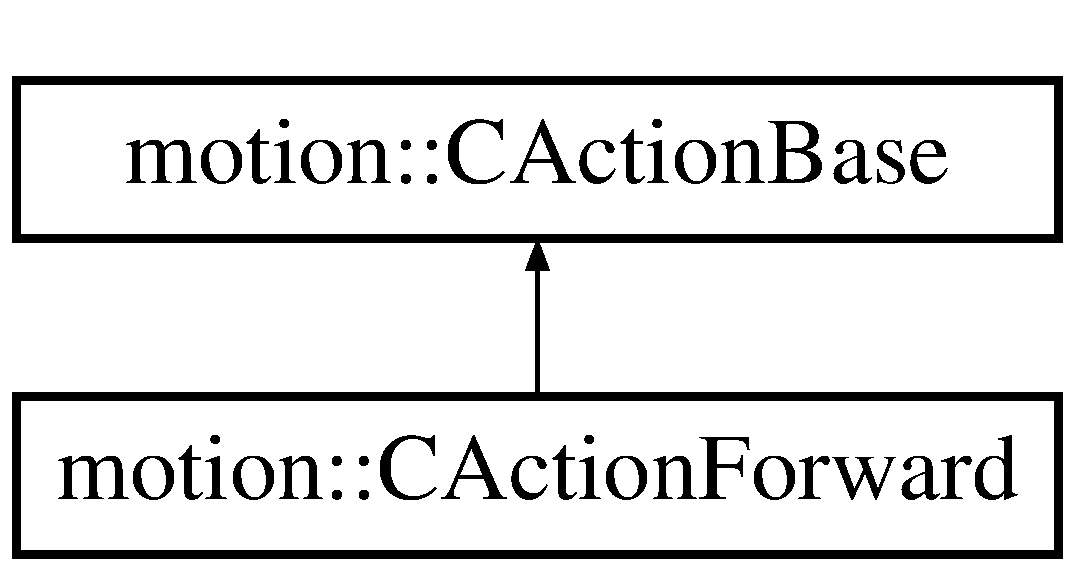
\includegraphics[height=2.000000cm]{classmotion_1_1CActionForward}
\end{center}
\end{figure}
\subsection*{Public Member Functions}
\begin{DoxyCompactItemize}
\item 
void \mbox{\hyperlink{classmotion_1_1CActionForward_af7c72ffee0c2f41c8608259ef3268f23}{reset}} (void)
\item 
\mbox{\Hypertarget{classmotion_1_1CActionForward_af986e75f2773dced403311b3e5e1d7b8}\label{classmotion_1_1CActionForward_af986e75f2773dced403311b3e5e1d7b8}} 
E\+Steering\+State\+Type {\bfseries get\+State} (void)
\item 
\mbox{\Hypertarget{classmotion_1_1CActionForward_a0a17ba177738541886131deca36c6bf1}\label{classmotion_1_1CActionForward_a0a17ba177738541886131deca36c6bf1}} 
void {\bfseries set\+State} (E\+Steering\+State\+Type state)
\item 
void \mbox{\hyperlink{classmotion_1_1CActionForward_abc4d3b39f49514f9d3f64a92393aa6d2}{forward}} (double v, double distance)
\end{DoxyCompactItemize}
\subsection*{Static Public Member Functions}
\begin{DoxyCompactItemize}
\item 
\mbox{\Hypertarget{classmotion_1_1CActionForward_a7820340aa671aaf37c16b945f023b82f}\label{classmotion_1_1CActionForward_a7820340aa671aaf37c16b945f023b82f}} 
static \mbox{\hyperlink{classmotion_1_1CActionForward}{C\+Action\+Forward}} $\ast$ {\bfseries get\+Instance} (void)
\end{DoxyCompactItemize}


\subsection{Member Function Documentation}
\mbox{\Hypertarget{classmotion_1_1CActionForward_abc4d3b39f49514f9d3f64a92393aa6d2}\label{classmotion_1_1CActionForward_abc4d3b39f49514f9d3f64a92393aa6d2}} 
\index{motion\+::\+C\+Action\+Forward@{motion\+::\+C\+Action\+Forward}!forward@{forward}}
\index{forward@{forward}!motion\+::\+C\+Action\+Forward@{motion\+::\+C\+Action\+Forward}}
\subsubsection{\texorpdfstring{forward()}{forward()}}
{\footnotesize\ttfamily void C\+Action\+Forward\+::forward (\begin{DoxyParamCaption}\item[{double}]{v,  }\item[{double}]{distance }\end{DoxyParamCaption})}

Move the robot forward straightly. 
\begin{DoxyParams}{Parameters}
{\em v} & is the forward linear velocity. \\
\hline
{\em distance} & is the desired distance we want the robot forward. \\
\hline
\end{DoxyParams}
start the timer \mbox{\Hypertarget{classmotion_1_1CActionForward_af7c72ffee0c2f41c8608259ef3268f23}\label{classmotion_1_1CActionForward_af7c72ffee0c2f41c8608259ef3268f23}} 
\index{motion\+::\+C\+Action\+Forward@{motion\+::\+C\+Action\+Forward}!reset@{reset}}
\index{reset@{reset}!motion\+::\+C\+Action\+Forward@{motion\+::\+C\+Action\+Forward}}
\subsubsection{\texorpdfstring{reset()}{reset()}}
{\footnotesize\ttfamily void C\+Action\+Forward\+::reset (\begin{DoxyParamCaption}\item[{void}]{ }\end{DoxyParamCaption})}

$<$ Reset base private variables. 

The documentation for this class was generated from the following files\+:\begin{DoxyCompactItemize}
\item 
motion/action/C\+Action\+Forward.\+h\item 
motion/action/C\+Action\+Forward.\+cpp\end{DoxyCompactItemize}

\hypertarget{classmotion_1_1CMotionWallFollowing}{}\section{motion\+:\+:C\+Motion\+Wall\+Following Class Reference}
\label{classmotion_1_1CMotionWallFollowing}\index{motion\+::\+C\+Motion\+Wall\+Following@{motion\+::\+C\+Motion\+Wall\+Following}}


{\ttfamily \#include $<$C\+Motion\+Wall\+Following.\+h$>$}

Inheritance diagram for motion\+:\+:C\+Motion\+Wall\+Following\+:\begin{figure}[H]
\begin{center}
\leavevmode
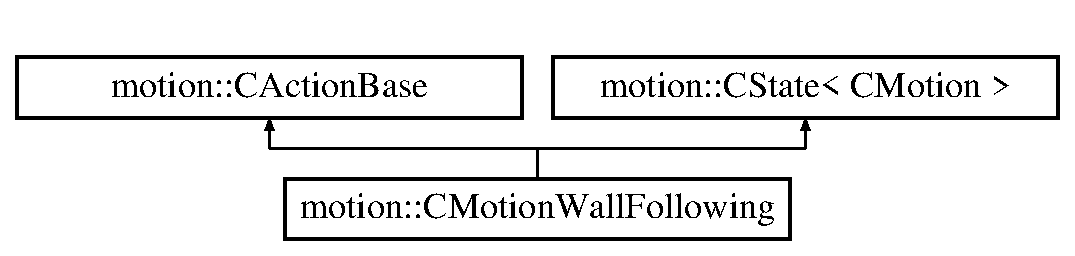
\includegraphics[height=2.000000cm]{classmotion_1_1CMotionWallFollowing}
\end{center}
\end{figure}
\subsection*{Public Member Functions}
\begin{DoxyCompactItemize}
\item 
virtual void \mbox{\hyperlink{classmotion_1_1CMotionWallFollowing_ad42584f648abe8826d2c23dad8128484}{enter}} (\mbox{\hyperlink{classmotion_1_1CMotion}{C\+Motion}} $\ast$mt)
\item 
virtual void \mbox{\hyperlink{classmotion_1_1CMotionWallFollowing_a765cfe604941a06056131feb01fea66d}{execute}} (\mbox{\hyperlink{classmotion_1_1CMotion}{C\+Motion}} $\ast$mt)
\item 
virtual void \mbox{\hyperlink{classmotion_1_1CMotionWallFollowing_a24be76c786b3a4bd476cc9b3c8955c26}{exit}} (\mbox{\hyperlink{classmotion_1_1CMotion}{C\+Motion}} $\ast$mt)
\item 
\mbox{\Hypertarget{classmotion_1_1CMotionWallFollowing_ab85ceaa8803a0850acdc951bd9ebec74}\label{classmotion_1_1CMotionWallFollowing_ab85ceaa8803a0850acdc951bd9ebec74}} 
void {\bfseries reset} (void)
\item 
\mbox{\Hypertarget{classmotion_1_1CMotionWallFollowing_a0ab894226ca05974580ec97ececbda5d}\label{classmotion_1_1CMotionWallFollowing_a0ab894226ca05974580ec97ececbda5d}} 
\mbox{\hyperlink{classmotion_1_1CStateMachine}{C\+State\+Machine}}$<$ \mbox{\hyperlink{classmotion_1_1CMotionWallFollowing}{C\+Motion\+Wall\+Following}} $>$ $\ast$ {\bfseries get\+F\+SM} (void) const
\item 
double \mbox{\hyperlink{classmotion_1_1CMotionWallFollowing_a1b29295eff775104bb16c110c3f8b81a}{tune\+Velocity}} (void)
\item 
double \mbox{\hyperlink{classmotion_1_1CMotionWallFollowing_ad8a39e0176c9e6127b8267b1a7a891ac}{calc\+Rem\+Angle}} (void)
\item 
bool \mbox{\hyperlink{classmotion_1_1CMotionWallFollowing_a4fcea1525cdd043f8c0dd8621e3ba09e}{dist\+Reached}} (void)
\item 
bool \mbox{\hyperlink{classmotion_1_1CMotionWallFollowing_aa84fb18a4cea89ad726c18d4f308e4d7}{ang\+N\+Dist\+Reached}} (void)
\end{DoxyCompactItemize}
\subsection*{Static Public Member Functions}
\begin{DoxyCompactItemize}
\item 
\mbox{\Hypertarget{classmotion_1_1CMotionWallFollowing_a8758349202ccb49d5b0927066b4201cd}\label{classmotion_1_1CMotionWallFollowing_a8758349202ccb49d5b0927066b4201cd}} 
static \mbox{\hyperlink{classmotion_1_1CMotionWallFollowing}{C\+Motion\+Wall\+Following}} $\ast$ {\bfseries get\+Instance} (void)
\end{DoxyCompactItemize}


\subsection{Detailed Description}
Wall following mode. Need the following linear velocity and the desired follow distance as input. 

\subsection{Member Function Documentation}
\mbox{\Hypertarget{classmotion_1_1CMotionWallFollowing_aa84fb18a4cea89ad726c18d4f308e4d7}\label{classmotion_1_1CMotionWallFollowing_aa84fb18a4cea89ad726c18d4f308e4d7}} 
\index{motion\+::\+C\+Motion\+Wall\+Following@{motion\+::\+C\+Motion\+Wall\+Following}!ang\+N\+Dist\+Reached@{ang\+N\+Dist\+Reached}}
\index{ang\+N\+Dist\+Reached@{ang\+N\+Dist\+Reached}!motion\+::\+C\+Motion\+Wall\+Following@{motion\+::\+C\+Motion\+Wall\+Following}}
\subsubsection{\texorpdfstring{ang\+N\+Dist\+Reached()}{angNDistReached()}}
{\footnotesize\ttfamily bool C\+Motion\+Wall\+Following\+::ang\+N\+Dist\+Reached (\begin{DoxyParamCaption}\item[{void}]{ }\end{DoxyParamCaption})}

The resume angle and distance satisfied or not. \begin{DoxyReturn}{Returns}
true if angle condition is satisfied and side distance is larger than obs\+Stop\+Dist. 
\end{DoxyReturn}
\begin{DoxySeeAlso}{See also}
\mbox{\hyperlink{classmotion_1_1CMotionWallFollowing_a4fcea1525cdd043f8c0dd8621e3ba09e}{dist\+Reached}} 

obs\+Stop\+Dist 
\end{DoxySeeAlso}
\mbox{\Hypertarget{classmotion_1_1CMotionWallFollowing_ad8a39e0176c9e6127b8267b1a7a891ac}\label{classmotion_1_1CMotionWallFollowing_ad8a39e0176c9e6127b8267b1a7a891ac}} 
\index{motion\+::\+C\+Motion\+Wall\+Following@{motion\+::\+C\+Motion\+Wall\+Following}!calc\+Rem\+Angle@{calc\+Rem\+Angle}}
\index{calc\+Rem\+Angle@{calc\+Rem\+Angle}!motion\+::\+C\+Motion\+Wall\+Following@{motion\+::\+C\+Motion\+Wall\+Following}}
\subsubsection{\texorpdfstring{calc\+Rem\+Angle()}{calcRemAngle()}}
{\footnotesize\ttfamily double C\+Motion\+Wall\+Following\+::calc\+Rem\+Angle (\begin{DoxyParamCaption}\item[{void}]{ }\end{DoxyParamCaption})}

Calculate remaining angle, when this angle approached 0, it means the angle condition of ang\+N\+Dist\+Reached is satisfied. \begin{DoxyReturn}{Returns}
Remaining angle. 
\end{DoxyReturn}
\begin{DoxySeeAlso}{See also}
\mbox{\hyperlink{classmotion_1_1CMotionWallFollowing_aa84fb18a4cea89ad726c18d4f308e4d7}{ang\+N\+Dist\+Reached}} 
\end{DoxySeeAlso}
return motion\+Absd(rad2\+Deg(m\+\_\+end\+Phi -\/ get\+Cur\+Pose().phi)); \mbox{\Hypertarget{classmotion_1_1CMotionWallFollowing_a4fcea1525cdd043f8c0dd8621e3ba09e}\label{classmotion_1_1CMotionWallFollowing_a4fcea1525cdd043f8c0dd8621e3ba09e}} 
\index{motion\+::\+C\+Motion\+Wall\+Following@{motion\+::\+C\+Motion\+Wall\+Following}!dist\+Reached@{dist\+Reached}}
\index{dist\+Reached@{dist\+Reached}!motion\+::\+C\+Motion\+Wall\+Following@{motion\+::\+C\+Motion\+Wall\+Following}}
\subsubsection{\texorpdfstring{dist\+Reached()}{distReached()}}
{\footnotesize\ttfamily bool C\+Motion\+Wall\+Following\+::dist\+Reached (\begin{DoxyParamCaption}\item[{void}]{ }\end{DoxyParamCaption})}

The resume distance satisfied or not. \begin{DoxyReturn}{Returns}
true if ahead distance is larger than wall\+Fol\+Resume\+Dist. 
\end{DoxyReturn}
\begin{DoxySeeAlso}{See also}
\mbox{\hyperlink{classmotion_1_1CMotionWallFollowing_aa84fb18a4cea89ad726c18d4f308e4d7}{ang\+N\+Dist\+Reached}} 

wall\+Fol\+Resume\+Dist 
\end{DoxySeeAlso}
\mbox{\Hypertarget{classmotion_1_1CMotionWallFollowing_ad42584f648abe8826d2c23dad8128484}\label{classmotion_1_1CMotionWallFollowing_ad42584f648abe8826d2c23dad8128484}} 
\index{motion\+::\+C\+Motion\+Wall\+Following@{motion\+::\+C\+Motion\+Wall\+Following}!enter@{enter}}
\index{enter@{enter}!motion\+::\+C\+Motion\+Wall\+Following@{motion\+::\+C\+Motion\+Wall\+Following}}
\subsubsection{\texorpdfstring{enter()}{enter()}}
{\footnotesize\ttfamily void C\+Motion\+Wall\+Following\+::enter (\begin{DoxyParamCaption}\item[{\mbox{\hyperlink{classmotion_1_1CMotion}{C\+Motion}} $\ast$}]{ }\end{DoxyParamCaption})\hspace{0.3cm}{\ttfamily [virtual]}}

This will execute when the state is entered. set\+Motion(\+W\+A\+L\+L\+\_\+\+F\+O\+L\+L\+O\+W\+I\+N\+G); 

Implements \mbox{\hyperlink{classmotion_1_1CState_a53d5fcfec223b58ccdd364a8430fd23c}{motion\+::\+C\+State$<$ C\+Motion $>$}}.

\mbox{\Hypertarget{classmotion_1_1CMotionWallFollowing_a765cfe604941a06056131feb01fea66d}\label{classmotion_1_1CMotionWallFollowing_a765cfe604941a06056131feb01fea66d}} 
\index{motion\+::\+C\+Motion\+Wall\+Following@{motion\+::\+C\+Motion\+Wall\+Following}!execute@{execute}}
\index{execute@{execute}!motion\+::\+C\+Motion\+Wall\+Following@{motion\+::\+C\+Motion\+Wall\+Following}}
\subsubsection{\texorpdfstring{execute()}{execute()}}
{\footnotesize\ttfamily void C\+Motion\+Wall\+Following\+::execute (\begin{DoxyParamCaption}\item[{\mbox{\hyperlink{classmotion_1_1CMotion}{C\+Motion}} $\ast$}]{ }\end{DoxyParamCaption})\hspace{0.3cm}{\ttfamily [virtual]}}

This is the states normal update function. 

Implements \mbox{\hyperlink{classmotion_1_1CState_a71dc72d345b15bf3b5b5bff596a71f33}{motion\+::\+C\+State$<$ C\+Motion $>$}}.

\mbox{\Hypertarget{classmotion_1_1CMotionWallFollowing_a24be76c786b3a4bd476cc9b3c8955c26}\label{classmotion_1_1CMotionWallFollowing_a24be76c786b3a4bd476cc9b3c8955c26}} 
\index{motion\+::\+C\+Motion\+Wall\+Following@{motion\+::\+C\+Motion\+Wall\+Following}!exit@{exit}}
\index{exit@{exit}!motion\+::\+C\+Motion\+Wall\+Following@{motion\+::\+C\+Motion\+Wall\+Following}}
\subsubsection{\texorpdfstring{exit()}{exit()}}
{\footnotesize\ttfamily void C\+Motion\+Wall\+Following\+::exit (\begin{DoxyParamCaption}\item[{\mbox{\hyperlink{classmotion_1_1CMotion}{C\+Motion}} $\ast$}]{ }\end{DoxyParamCaption})\hspace{0.3cm}{\ttfamily [virtual]}}

This will execute when the state is exited. 

Implements \mbox{\hyperlink{classmotion_1_1CState_a353db064c159d66b82bf257b35e7c016}{motion\+::\+C\+State$<$ C\+Motion $>$}}.

\mbox{\Hypertarget{classmotion_1_1CMotionWallFollowing_a1b29295eff775104bb16c110c3f8b81a}\label{classmotion_1_1CMotionWallFollowing_a1b29295eff775104bb16c110c3f8b81a}} 
\index{motion\+::\+C\+Motion\+Wall\+Following@{motion\+::\+C\+Motion\+Wall\+Following}!tune\+Velocity@{tune\+Velocity}}
\index{tune\+Velocity@{tune\+Velocity}!motion\+::\+C\+Motion\+Wall\+Following@{motion\+::\+C\+Motion\+Wall\+Following}}
\subsubsection{\texorpdfstring{tune\+Velocity()}{tuneVelocity()}}
{\footnotesize\ttfamily double C\+Motion\+Wall\+Following\+::tune\+Velocity (\begin{DoxyParamCaption}\item[{void}]{ }\end{DoxyParamCaption})}

Tune the velocity according to the distance from robot to wall. \begin{DoxyReturn}{Returns}
The scale that velocity should be Tuned. It\textquotesingle{}s a ratio between 0 and 1. 
\end{DoxyReturn}


The documentation for this class was generated from the following files\+:\begin{DoxyCompactItemize}
\item 
motion/\mbox{\hyperlink{CMotionWallFollowing_8h}{C\+Motion\+Wall\+Following.\+h}}\item 
motion/\mbox{\hyperlink{CMotionWallFollowing_8cpp}{C\+Motion\+Wall\+Following.\+cpp}}\end{DoxyCompactItemize}

\hypertarget{classCMyGLCanvas}{}\section{C\+My\+G\+L\+Canvas Class Reference}
\label{classCMyGLCanvas}\index{C\+My\+G\+L\+Canvas@{C\+My\+G\+L\+Canvas}}
Inheritance diagram for C\+My\+G\+L\+Canvas\+:\begin{figure}[H]
\begin{center}
\leavevmode
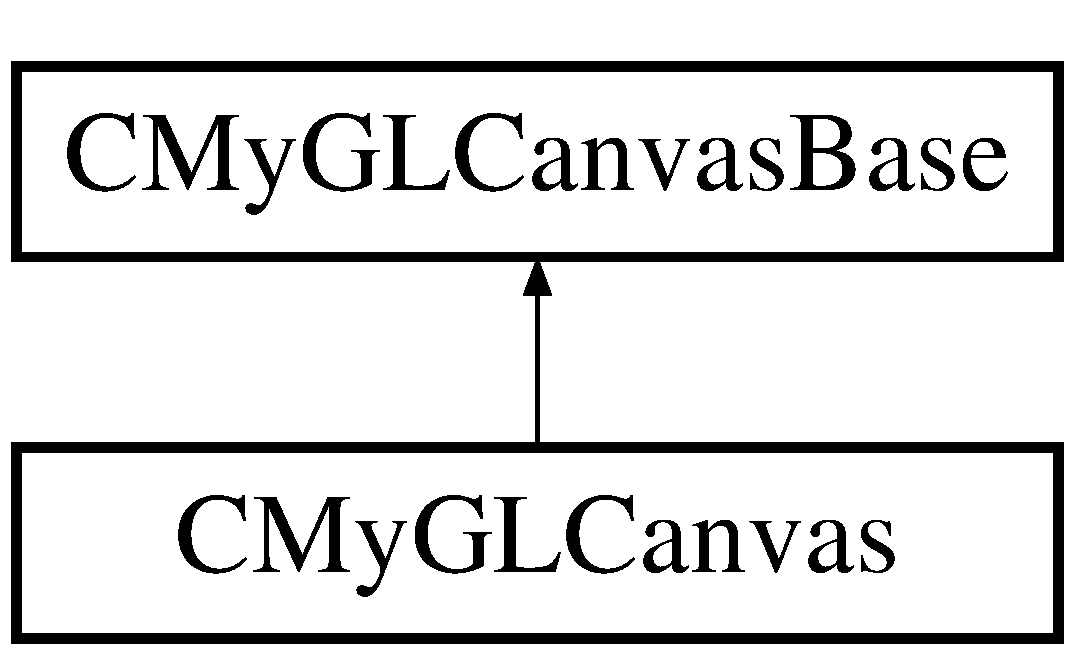
\includegraphics[height=2.000000cm]{classCMyGLCanvas}
\end{center}
\end{figure}
\subsection*{Public Member Functions}
\begin{DoxyCompactItemize}
\item 
\mbox{\Hypertarget{classCMyGLCanvas_a2444e5482d703a8d81d138cd2fb5d275}\label{classCMyGLCanvas_a2444e5482d703a8d81d138cd2fb5d275}} 
{\bfseries C\+My\+G\+L\+Canvas} (wx\+Window $\ast$parent, wx\+Window\+ID id=wx\+I\+D\+\_\+\+A\+NY, const wx\+Point \&pos=wx\+Default\+Position, const wx\+Size \&size=wx\+Default\+Size, long style=0, const wx\+String \&name=\+\_\+T(\char`\"{}C\+My\+G\+L\+Canvas\+Base\char`\"{}))
\item 
\mbox{\Hypertarget{classCMyGLCanvas_a136b603a8e7561bbdf15085daf349687}\label{classCMyGLCanvas_a136b603a8e7561bbdf15085daf349687}} 
void {\bfseries On\+Char\+Custom} (wx\+Key\+Event \&event)
\item 
\mbox{\Hypertarget{classCMyGLCanvas_a99b67a508a8603e6c5cf0856e9353bf6}\label{classCMyGLCanvas_a99b67a508a8603e6c5cf0856e9353bf6}} 
void {\bfseries On\+Pre\+Render} ()
\item 
\mbox{\Hypertarget{classCMyGLCanvas_aef8ded22cd9ecac73ad52c0ac6af46e1}\label{classCMyGLCanvas_aef8ded22cd9ecac73ad52c0ac6af46e1}} 
void {\bfseries On\+Post\+Render} ()
\item 
\mbox{\Hypertarget{classCMyGLCanvas_a4be08ca79a2f75ee1a142f136307dc57}\label{classCMyGLCanvas_a4be08ca79a2f75ee1a142f136307dc57}} 
void {\bfseries On\+Post\+Render\+Swap\+Buffers} (double At, wx\+Paint\+DC \&dc)
\item 
\mbox{\Hypertarget{classCMyGLCanvas_a33d6dfb37f2d4f11237a3c547d683047}\label{classCMyGLCanvas_a33d6dfb37f2d4f11237a3c547d683047}} 
void {\bfseries On\+Render\+Error} (const wx\+String \&str)
\end{DoxyCompactItemize}


The documentation for this class was generated from the following file\+:\begin{DoxyCompactItemize}
\item 
gridmap\+Simul\+Main.\+cpp\end{DoxyCompactItemize}

\hypertarget{classmotion_1_1CState}{}\section{motion\+:\+:C\+State$<$ state\+\_\+type $>$ Class Template Reference}
\label{classmotion_1_1CState}\index{motion\+::\+C\+State$<$ state\+\_\+type $>$@{motion\+::\+C\+State$<$ state\+\_\+type $>$}}
\subsection*{Public Member Functions}
\begin{DoxyCompactItemize}
\item 
virtual void \mbox{\hyperlink{classmotion_1_1CState_a53d5fcfec223b58ccdd364a8430fd23c}{enter}} (state\+\_\+type $\ast$)=0
\item 
virtual void \mbox{\hyperlink{classmotion_1_1CState_a71dc72d345b15bf3b5b5bff596a71f33}{execute}} (state\+\_\+type $\ast$)=0
\item 
virtual void \mbox{\hyperlink{classmotion_1_1CState_a353db064c159d66b82bf257b35e7c016}{exit}} (state\+\_\+type $\ast$)=0
\end{DoxyCompactItemize}


\subsection{Member Function Documentation}
\mbox{\Hypertarget{classmotion_1_1CState_a53d5fcfec223b58ccdd364a8430fd23c}\label{classmotion_1_1CState_a53d5fcfec223b58ccdd364a8430fd23c}} 
\index{motion\+::\+C\+State@{motion\+::\+C\+State}!enter@{enter}}
\index{enter@{enter}!motion\+::\+C\+State@{motion\+::\+C\+State}}
\subsubsection{\texorpdfstring{enter()}{enter()}}
{\footnotesize\ttfamily template$<$class state\+\_\+type$>$ \\
virtual void \mbox{\hyperlink{classmotion_1_1CState}{motion\+::\+C\+State}}$<$ state\+\_\+type $>$\+::enter (\begin{DoxyParamCaption}\item[{state\+\_\+type $\ast$}]{ }\end{DoxyParamCaption})\hspace{0.3cm}{\ttfamily [pure virtual]}}

This will execute when the state is entered. \mbox{\Hypertarget{classmotion_1_1CState_a71dc72d345b15bf3b5b5bff596a71f33}\label{classmotion_1_1CState_a71dc72d345b15bf3b5b5bff596a71f33}} 
\index{motion\+::\+C\+State@{motion\+::\+C\+State}!execute@{execute}}
\index{execute@{execute}!motion\+::\+C\+State@{motion\+::\+C\+State}}
\subsubsection{\texorpdfstring{execute()}{execute()}}
{\footnotesize\ttfamily template$<$class state\+\_\+type$>$ \\
virtual void \mbox{\hyperlink{classmotion_1_1CState}{motion\+::\+C\+State}}$<$ state\+\_\+type $>$\+::execute (\begin{DoxyParamCaption}\item[{state\+\_\+type $\ast$}]{ }\end{DoxyParamCaption})\hspace{0.3cm}{\ttfamily [pure virtual]}}

This is the states normal update function. \mbox{\Hypertarget{classmotion_1_1CState_a353db064c159d66b82bf257b35e7c016}\label{classmotion_1_1CState_a353db064c159d66b82bf257b35e7c016}} 
\index{motion\+::\+C\+State@{motion\+::\+C\+State}!exit@{exit}}
\index{exit@{exit}!motion\+::\+C\+State@{motion\+::\+C\+State}}
\subsubsection{\texorpdfstring{exit()}{exit()}}
{\footnotesize\ttfamily template$<$class state\+\_\+type$>$ \\
virtual void \mbox{\hyperlink{classmotion_1_1CState}{motion\+::\+C\+State}}$<$ state\+\_\+type $>$\+::exit (\begin{DoxyParamCaption}\item[{state\+\_\+type $\ast$}]{ }\end{DoxyParamCaption})\hspace{0.3cm}{\ttfamily [pure virtual]}}

This will execute when the state is exited. 

The documentation for this class was generated from the following file\+:\begin{DoxyCompactItemize}
\item 
motion/C\+State.\+h\end{DoxyCompactItemize}

\hypertarget{classmotion_1_1CStateMachine}{}\section{motion\+:\+:C\+State\+Machine$<$ state\+\_\+type $>$ Class Template Reference}
\label{classmotion_1_1CStateMachine}\index{motion\+::\+C\+State\+Machine$<$ state\+\_\+type $>$@{motion\+::\+C\+State\+Machine$<$ state\+\_\+type $>$}}
\subsection*{Public Member Functions}
\begin{DoxyCompactItemize}
\item 
\mbox{\Hypertarget{classmotion_1_1CStateMachine_ac91f606bd5d004771294c02a3990f7ed}\label{classmotion_1_1CStateMachine_ac91f606bd5d004771294c02a3990f7ed}} 
{\bfseries C\+State\+Machine} (state\+\_\+type $\ast$owner)
\item 
void \mbox{\hyperlink{classmotion_1_1CStateMachine_a57407660e1054b7b6e912efc3afb9495}{set\+Current\+State}} (\mbox{\hyperlink{classmotion_1_1CState}{C\+State}}$<$ state\+\_\+type $>$ $\ast$s)
\item 
\mbox{\Hypertarget{classmotion_1_1CStateMachine_aaeead01662f75ed768226163665bcec4}\label{classmotion_1_1CStateMachine_aaeead01662f75ed768226163665bcec4}} 
void {\bfseries set\+Global\+State} (\mbox{\hyperlink{classmotion_1_1CState}{C\+State}}$<$ state\+\_\+type $>$ $\ast$s)
\item 
\mbox{\Hypertarget{classmotion_1_1CStateMachine_a55764d2e385cb61f26e6aa09f80577e4}\label{classmotion_1_1CStateMachine_a55764d2e385cb61f26e6aa09f80577e4}} 
void {\bfseries set\+Previous\+State} (\mbox{\hyperlink{classmotion_1_1CState}{C\+State}}$<$ state\+\_\+type $>$ $\ast$s)
\item 
void \mbox{\hyperlink{classmotion_1_1CStateMachine_a8a944b6b5dcff9b614b434fabcd8955c}{update}} () const
\item 
void \mbox{\hyperlink{classmotion_1_1CStateMachine_a13d97b778f850709c7f9060de4aba142}{change\+State}} (\mbox{\hyperlink{classmotion_1_1CState}{C\+State}}$<$ state\+\_\+type $>$ $\ast$p\+New\+State)
\item 
void \mbox{\hyperlink{classmotion_1_1CStateMachine_ae8e1d802793aded65b1da25dad007486}{revert\+To\+Previous\+State}} ()
\item 
\mbox{\hyperlink{classmotion_1_1CState}{C\+State}}$<$ state\+\_\+type $>$ $\ast$ \mbox{\hyperlink{classmotion_1_1CStateMachine_a2231e1232b1fe6a793b95e0e2217f362}{get\+Current\+State}} (void) const
\item 
\mbox{\Hypertarget{classmotion_1_1CStateMachine_ac9e635be4cb960479c6cdef54966480b}\label{classmotion_1_1CStateMachine_ac9e635be4cb960479c6cdef54966480b}} 
\mbox{\hyperlink{classmotion_1_1CState}{C\+State}}$<$ state\+\_\+type $>$ $\ast$ {\bfseries get\+Global\+State} (void) const
\item 
\mbox{\Hypertarget{classmotion_1_1CStateMachine_acab2aefef8b1fa57d211eb68aa8e96f8}\label{classmotion_1_1CStateMachine_acab2aefef8b1fa57d211eb68aa8e96f8}} 
\mbox{\hyperlink{classmotion_1_1CState}{C\+State}}$<$ state\+\_\+type $>$ $\ast$ {\bfseries get\+Previous\+State} (void) const
\end{DoxyCompactItemize}


\subsection{Member Function Documentation}
\mbox{\Hypertarget{classmotion_1_1CStateMachine_a13d97b778f850709c7f9060de4aba142}\label{classmotion_1_1CStateMachine_a13d97b778f850709c7f9060de4aba142}} 
\index{motion\+::\+C\+State\+Machine@{motion\+::\+C\+State\+Machine}!change\+State@{change\+State}}
\index{change\+State@{change\+State}!motion\+::\+C\+State\+Machine@{motion\+::\+C\+State\+Machine}}
\subsubsection{\texorpdfstring{change\+State()}{changeState()}}
{\footnotesize\ttfamily template$<$class state\+\_\+type$>$ \\
void \mbox{\hyperlink{classmotion_1_1CStateMachine}{motion\+::\+C\+State\+Machine}}$<$ state\+\_\+type $>$\+::change\+State (\begin{DoxyParamCaption}\item[{\mbox{\hyperlink{classmotion_1_1CState}{C\+State}}$<$ state\+\_\+type $>$ $\ast$}]{p\+New\+State }\end{DoxyParamCaption})\hspace{0.3cm}{\ttfamily [inline]}}

Change to a new state. Keep a record of the previous state. ~\newline
~\newline
~\newline
 Call the exit method of the existing state. ~\newline
~\newline
 Change state to the new state. ~\newline
 Call the entry method of the new state. \mbox{\Hypertarget{classmotion_1_1CStateMachine_a2231e1232b1fe6a793b95e0e2217f362}\label{classmotion_1_1CStateMachine_a2231e1232b1fe6a793b95e0e2217f362}} 
\index{motion\+::\+C\+State\+Machine@{motion\+::\+C\+State\+Machine}!get\+Current\+State@{get\+Current\+State}}
\index{get\+Current\+State@{get\+Current\+State}!motion\+::\+C\+State\+Machine@{motion\+::\+C\+State\+Machine}}
\subsubsection{\texorpdfstring{get\+Current\+State()}{getCurrentState()}}
{\footnotesize\ttfamily template$<$class state\+\_\+type$>$ \\
\mbox{\hyperlink{classmotion_1_1CState}{C\+State}}$<$state\+\_\+type$>$$\ast$ \mbox{\hyperlink{classmotion_1_1CStateMachine}{motion\+::\+C\+State\+Machine}}$<$ state\+\_\+type $>$\+::get\+Current\+State (\begin{DoxyParamCaption}\item[{void}]{ }\end{DoxyParamCaption}) const\hspace{0.3cm}{\ttfamily [inline]}}

Returns true if the current state\textquotesingle{}s type is equal to the type of the class passed as a parameter.\+bool is\+In\+State(const C\+State$<$state\+\_\+type$>$\& st) const \{ return typeid($\ast$m\+\_\+p\+Current\+State) == typeid(st); \} \mbox{\Hypertarget{classmotion_1_1CStateMachine_ae8e1d802793aded65b1da25dad007486}\label{classmotion_1_1CStateMachine_ae8e1d802793aded65b1da25dad007486}} 
\index{motion\+::\+C\+State\+Machine@{motion\+::\+C\+State\+Machine}!revert\+To\+Previous\+State@{revert\+To\+Previous\+State}}
\index{revert\+To\+Previous\+State@{revert\+To\+Previous\+State}!motion\+::\+C\+State\+Machine@{motion\+::\+C\+State\+Machine}}
\subsubsection{\texorpdfstring{revert\+To\+Previous\+State()}{revertToPreviousState()}}
{\footnotesize\ttfamily template$<$class state\+\_\+type$>$ \\
void \mbox{\hyperlink{classmotion_1_1CStateMachine}{motion\+::\+C\+State\+Machine}}$<$ state\+\_\+type $>$\+::revert\+To\+Previous\+State (\begin{DoxyParamCaption}{ }\end{DoxyParamCaption})\hspace{0.3cm}{\ttfamily [inline]}}

Change state back to the previous state. \mbox{\Hypertarget{classmotion_1_1CStateMachine_a57407660e1054b7b6e912efc3afb9495}\label{classmotion_1_1CStateMachine_a57407660e1054b7b6e912efc3afb9495}} 
\index{motion\+::\+C\+State\+Machine@{motion\+::\+C\+State\+Machine}!set\+Current\+State@{set\+Current\+State}}
\index{set\+Current\+State@{set\+Current\+State}!motion\+::\+C\+State\+Machine@{motion\+::\+C\+State\+Machine}}
\subsubsection{\texorpdfstring{set\+Current\+State()}{setCurrentState()}}
{\footnotesize\ttfamily template$<$class state\+\_\+type$>$ \\
void \mbox{\hyperlink{classmotion_1_1CStateMachine}{motion\+::\+C\+State\+Machine}}$<$ state\+\_\+type $>$\+::set\+Current\+State (\begin{DoxyParamCaption}\item[{\mbox{\hyperlink{classmotion_1_1CState}{C\+State}}$<$ state\+\_\+type $>$ $\ast$}]{s }\end{DoxyParamCaption})\hspace{0.3cm}{\ttfamily [inline]}}

Use these methods to initialize the F\+SM. \mbox{\Hypertarget{classmotion_1_1CStateMachine_a8a944b6b5dcff9b614b434fabcd8955c}\label{classmotion_1_1CStateMachine_a8a944b6b5dcff9b614b434fabcd8955c}} 
\index{motion\+::\+C\+State\+Machine@{motion\+::\+C\+State\+Machine}!update@{update}}
\index{update@{update}!motion\+::\+C\+State\+Machine@{motion\+::\+C\+State\+Machine}}
\subsubsection{\texorpdfstring{update()}{update()}}
{\footnotesize\ttfamily template$<$class state\+\_\+type$>$ \\
void \mbox{\hyperlink{classmotion_1_1CStateMachine}{motion\+::\+C\+State\+Machine}}$<$ state\+\_\+type $>$\+::update (\begin{DoxyParamCaption}\item[{void}]{ }\end{DoxyParamCaption}) const\hspace{0.3cm}{\ttfamily [inline]}}

Call this to update the F\+SM. If a global state exists, call its execute method, else do nothing. ~\newline
~\newline
 if(m\+\_\+p\+Global\+State) m\+\_\+p\+Global\+State-\/$>$execute(m\+\_\+p\+Owner);

Same for the current state. 

The documentation for this class was generated from the following file\+:\begin{DoxyCompactItemize}
\item 
motion/\mbox{\hyperlink{CStateMachine_8h}{C\+State\+Machine.\+h}}\end{DoxyCompactItemize}

\hypertarget{classgridmapSimulApp}{}\section{gridmap\+Simul\+App Class Reference}
\label{classgridmapSimulApp}\index{gridmap\+Simul\+App@{gridmap\+Simul\+App}}
Inheritance diagram for gridmap\+Simul\+App\+:\begin{figure}[H]
\begin{center}
\leavevmode
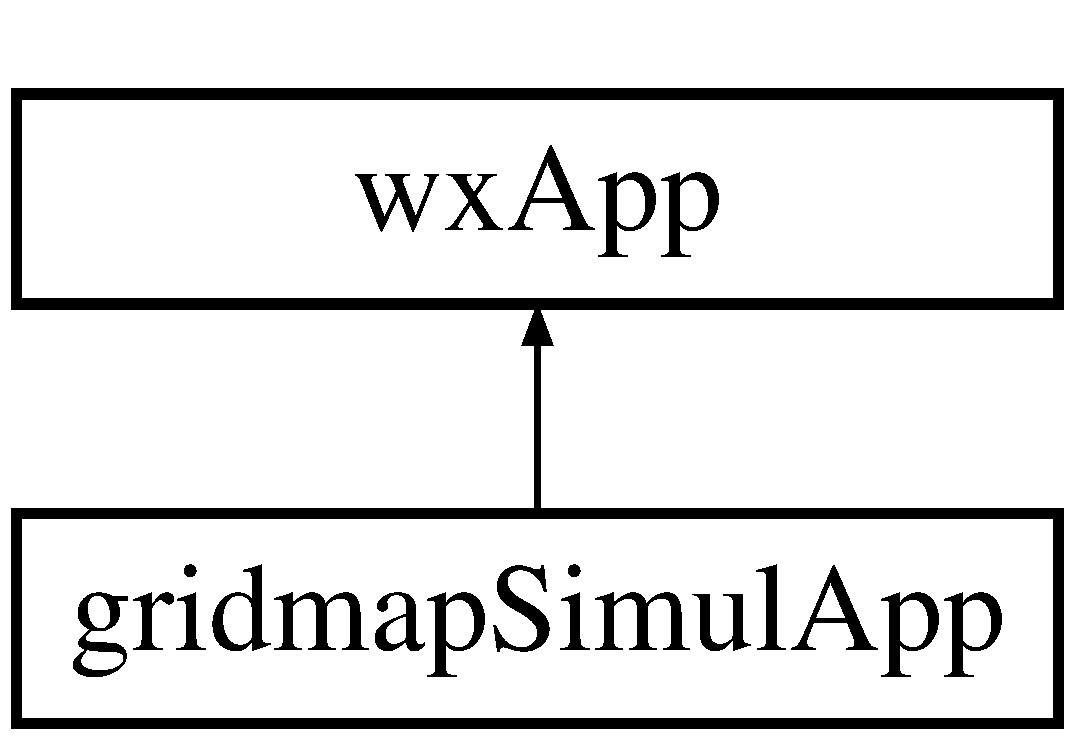
\includegraphics[height=2.000000cm]{classgridmapSimulApp}
\end{center}
\end{figure}
\subsection*{Public Member Functions}
\begin{DoxyCompactItemize}
\item 
\mbox{\Hypertarget{classgridmapSimulApp_abc43c8f695eb785e35a33f72ac180321}\label{classgridmapSimulApp_abc43c8f695eb785e35a33f72ac180321}} 
virtual bool {\bfseries On\+Init} ()
\item 
\mbox{\Hypertarget{classgridmapSimulApp_a4f8e8dc4a836ed655bde844103969e68}\label{classgridmapSimulApp_a4f8e8dc4a836ed655bde844103969e68}} 
virtual int {\bfseries On\+Exit} ()
\end{DoxyCompactItemize}


The documentation for this class was generated from the following files\+:\begin{DoxyCompactItemize}
\item 
gridmap\+Simul\+App.\+h\item 
gridmap\+Simul\+App.\+cpp\end{DoxyCompactItemize}

\hypertarget{classgridmapSimulFrame}{}\section{gridmap\+Simul\+Frame Class Reference}
\label{classgridmapSimulFrame}\index{gridmap\+Simul\+Frame@{gridmap\+Simul\+Frame}}
Inheritance diagram for gridmap\+Simul\+Frame\+:\begin{figure}[H]
\begin{center}
\leavevmode
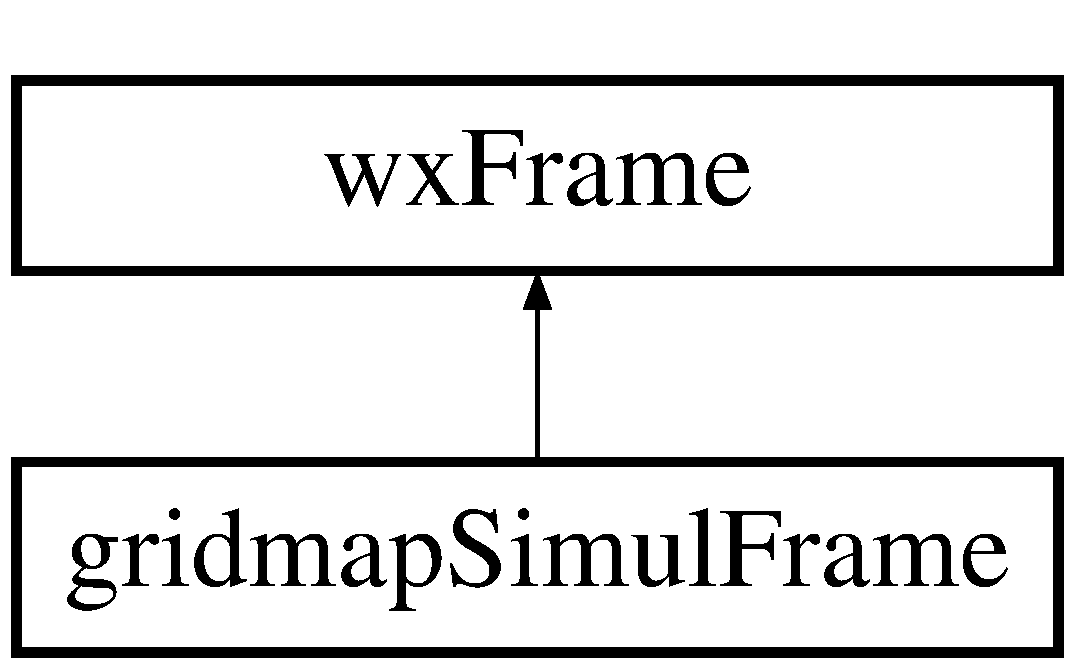
\includegraphics[height=2.000000cm]{classgridmapSimulFrame}
\end{center}
\end{figure}
\subsection*{Public Member Functions}
\begin{DoxyCompactItemize}
\item 
\mbox{\Hypertarget{classgridmapSimulFrame_ac1ac89ea6a9a31594031b1555124e9de}\label{classgridmapSimulFrame_ac1ac89ea6a9a31594031b1555124e9de}} 
{\bfseries gridmap\+Simul\+Frame} (wx\+Window $\ast$parent, wx\+Window\+ID id=-\/1)
\end{DoxyCompactItemize}


The documentation for this class was generated from the following files\+:\begin{DoxyCompactItemize}
\item 
gridmap\+Simul\+Main.\+h\item 
gridmap\+Simul\+Main.\+cpp\end{DoxyCompactItemize}

\hypertarget{classMyArtProvider}{}\section{My\+Art\+Provider Class Reference}
\label{classMyArtProvider}\index{My\+Art\+Provider@{My\+Art\+Provider}}
Inheritance diagram for My\+Art\+Provider\+:\begin{figure}[H]
\begin{center}
\leavevmode
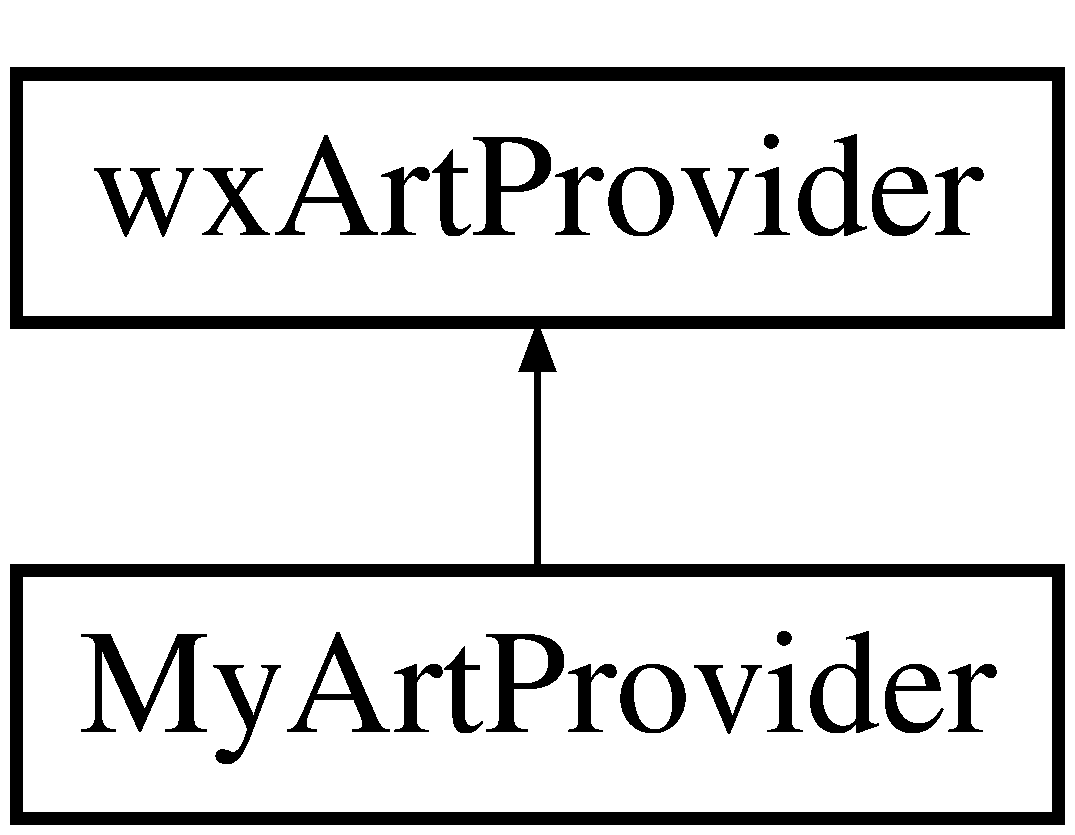
\includegraphics[height=2.000000cm]{classMyArtProvider}
\end{center}
\end{figure}
\subsection*{Protected Member Functions}
\begin{DoxyCompactItemize}
\item 
\mbox{\Hypertarget{classMyArtProvider_a4f06bcde38b57c560d5d9ec79ebd35dc}\label{classMyArtProvider_a4f06bcde38b57c560d5d9ec79ebd35dc}} 
virtual wx\+Bitmap {\bfseries Create\+Bitmap} (const wx\+Art\+ID \&id, const wx\+Art\+Client \&client, const wx\+Size \&size)
\end{DoxyCompactItemize}


\subsection{Detailed Description}
\#include \char`\"{}virtual\+\_\+map1.\+xpm\char`\"{} include \char`\"{}map2.\+xpm\char`\"{} include \char`\"{}map3.\+xpm\char`\"{} include \char`\"{}map3pro.\+xpm\char`\"{} \#include \char`\"{}map3pro\+\_\+mini\+\_\+xpm\char`\"{} include \char`\"{}map3pro\+\_\+mini2.\+xpm\char`\"{} 

The documentation for this class was generated from the following file\+:\begin{DoxyCompactItemize}
\item 
gridmap\+Simul\+Main.\+cpp\end{DoxyCompactItemize}

\hypertarget{structmotion_1_1TMotionPose2D}{}\section{motion\+:\+:T\+Motion\+Pose2D Struct Reference}
\label{structmotion_1_1TMotionPose2D}\index{motion\+::\+T\+Motion\+Pose2D@{motion\+::\+T\+Motion\+Pose2D}}
\subsection*{Public Member Functions}
\begin{DoxyCompactItemize}
\item 
\mbox{\Hypertarget{structmotion_1_1TMotionPose2D_a95c04345793f02fbc32792a9739d754d}\label{structmotion_1_1TMotionPose2D_a95c04345793f02fbc32792a9739d754d}} 
{\bfseries T\+Motion\+Pose2D} (double xx, double yy, double pphi)
\item 
\mbox{\Hypertarget{structmotion_1_1TMotionPose2D_ae2879a58d5ba238d4137a049170cda83}\label{structmotion_1_1TMotionPose2D_ae2879a58d5ba238d4137a049170cda83}} 
const \mbox{\hyperlink{structmotion_1_1TMotionPose2D}{T\+Motion\+Pose2D}} \& {\bfseries operator=} (const \mbox{\hyperlink{structmotion_1_1TMotionPose2D}{T\+Motion\+Pose2D}} \&rhs)
\item 
\mbox{\Hypertarget{structmotion_1_1TMotionPose2D_ac678e92a153d2f21f2967846ce2a128e}\label{structmotion_1_1TMotionPose2D_ac678e92a153d2f21f2967846ce2a128e}} 
\mbox{\hyperlink{structmotion_1_1TMotionPose2D}{T\+Motion\+Pose2D}} {\bfseries operator+} (const \mbox{\hyperlink{structmotion_1_1TMotionPose2D}{T\+Motion\+Pose2D}} \&rhs)
\item 
\mbox{\Hypertarget{structmotion_1_1TMotionPose2D_ada5c57be32bc815786bbd377e4db8b1d}\label{structmotion_1_1TMotionPose2D_ada5c57be32bc815786bbd377e4db8b1d}} 
\mbox{\hyperlink{structmotion_1_1TMotionPose2D}{T\+Motion\+Pose2D}} {\bfseries operator-\/} (const \mbox{\hyperlink{structmotion_1_1TMotionPose2D}{T\+Motion\+Pose2D}} \&rhs)
\item 
\mbox{\Hypertarget{structmotion_1_1TMotionPose2D_a528b2418d8a4ebcbc5c8e3e0d160b66a}\label{structmotion_1_1TMotionPose2D_a528b2418d8a4ebcbc5c8e3e0d160b66a}} 
void {\bfseries reset} (void)
\end{DoxyCompactItemize}
\subsection*{Public Attributes}
\begin{DoxyCompactItemize}
\item 
\mbox{\Hypertarget{structmotion_1_1TMotionPose2D_a13a051574ba46d53cf3cf75d1fd12ea6}\label{structmotion_1_1TMotionPose2D_a13a051574ba46d53cf3cf75d1fd12ea6}} 
double {\bfseries x}
\item 
\mbox{\Hypertarget{structmotion_1_1TMotionPose2D_aa00ac7540cebe1e39f7a27961719ad72}\label{structmotion_1_1TMotionPose2D_aa00ac7540cebe1e39f7a27961719ad72}} 
double {\bfseries y}
\item 
\mbox{\Hypertarget{structmotion_1_1TMotionPose2D_a4bf517b21f755bcb7fe0f938eaaad3ee}\label{structmotion_1_1TMotionPose2D_a4bf517b21f755bcb7fe0f938eaaad3ee}} 
double {\bfseries phi}
\end{DoxyCompactItemize}


The documentation for this struct was generated from the following file\+:\begin{DoxyCompactItemize}
\item 
motion/misc/T\+Motion\+Pose2\+D.\+h\end{DoxyCompactItemize}

\hypertarget{structVector2D}{}\section{Vector2D Struct Reference}
\label{structVector2D}\index{Vector2D@{Vector2D}}
\subsection*{Public Member Functions}
\begin{DoxyCompactItemize}
\item 
\mbox{\Hypertarget{structVector2D_a5a6dfe0c8c79626b485c7a17e964c692}\label{structVector2D_a5a6dfe0c8c79626b485c7a17e964c692}} 
{\bfseries Vector2D} (double a, double b)
\item 
\mbox{\Hypertarget{structVector2D_a0f80d7fc49a21f3f0e414300ec033ce6}\label{structVector2D_a0f80d7fc49a21f3f0e414300ec033ce6}} 
void {\bfseries Zero} ()
\item 
\mbox{\Hypertarget{structVector2D_af368803cca03d8daa572f3f23e68453a}\label{structVector2D_af368803cca03d8daa572f3f23e68453a}} 
bool {\bfseries is\+Zero} () const
\item 
\mbox{\Hypertarget{structVector2D_adf941f3e417b6dfe737bc800800149af}\label{structVector2D_adf941f3e417b6dfe737bc800800149af}} 
double {\bfseries Length} () const
\item 
\mbox{\Hypertarget{structVector2D_a1c8aefc20c23520837a1d0268b028884}\label{structVector2D_a1c8aefc20c23520837a1d0268b028884}} 
double {\bfseries Length\+Sq} () const
\item 
\mbox{\Hypertarget{structVector2D_ac68f4dafca1639747c67c1b01e3a9f28}\label{structVector2D_ac68f4dafca1639747c67c1b01e3a9f28}} 
void {\bfseries Normalize} ()
\item 
\mbox{\Hypertarget{structVector2D_ad2f2dc12faf5165413b379e48bd83e06}\label{structVector2D_ad2f2dc12faf5165413b379e48bd83e06}} 
double {\bfseries Dot} (const \mbox{\hyperlink{structVector2D}{Vector2D}} \&v2) const
\item 
\mbox{\Hypertarget{structVector2D_a89b83b3346369eb59d1cce0966621f2d}\label{structVector2D_a89b83b3346369eb59d1cce0966621f2d}} 
int {\bfseries Sign} (const \mbox{\hyperlink{structVector2D}{Vector2D}} \&v2) const
\item 
\mbox{\Hypertarget{structVector2D_a5a96e4095069b9a0ccad27d918031e5b}\label{structVector2D_a5a96e4095069b9a0ccad27d918031e5b}} 
\mbox{\hyperlink{structVector2D}{Vector2D}} {\bfseries Perp} () const
\item 
\mbox{\Hypertarget{structVector2D_a005fda83f3daaf3458d68ec177caedfd}\label{structVector2D_a005fda83f3daaf3458d68ec177caedfd}} 
void {\bfseries Truncate} (double max)
\item 
\mbox{\Hypertarget{structVector2D_a7e637c70522b98cabe95f88276238e46}\label{structVector2D_a7e637c70522b98cabe95f88276238e46}} 
double {\bfseries Distance} (const \mbox{\hyperlink{structVector2D}{Vector2D}} \&v2) const
\item 
\mbox{\Hypertarget{structVector2D_a24f4bf1e423224a2d23840eecbdf34cd}\label{structVector2D_a24f4bf1e423224a2d23840eecbdf34cd}} 
double {\bfseries Distance\+Sq} (const \mbox{\hyperlink{structVector2D}{Vector2D}} \&v2) const
\item 
\mbox{\Hypertarget{structVector2D_a7cef865849390244f0e6f3dde552d27d}\label{structVector2D_a7cef865849390244f0e6f3dde552d27d}} 
void {\bfseries Reflect} (const \mbox{\hyperlink{structVector2D}{Vector2D}} \&norm)
\item 
\mbox{\Hypertarget{structVector2D_a26e417c30dcd5b7df9d0d909fdae97e4}\label{structVector2D_a26e417c30dcd5b7df9d0d909fdae97e4}} 
\mbox{\hyperlink{structVector2D}{Vector2D}} {\bfseries Get\+Reverse} () const
\item 
\mbox{\Hypertarget{structVector2D_aad76999952386d0e849237724e1c3781}\label{structVector2D_aad76999952386d0e849237724e1c3781}} 
const \mbox{\hyperlink{structVector2D}{Vector2D}} \& {\bfseries operator+=} (const \mbox{\hyperlink{structVector2D}{Vector2D}} \&rhs)
\item 
\mbox{\Hypertarget{structVector2D_a9ca1113d9f97c9f98fa08253ed164196}\label{structVector2D_a9ca1113d9f97c9f98fa08253ed164196}} 
const \mbox{\hyperlink{structVector2D}{Vector2D}} \& {\bfseries operator-\/=} (const \mbox{\hyperlink{structVector2D}{Vector2D}} \&rhs)
\item 
\mbox{\Hypertarget{structVector2D_a8c932cad899a6a37ddc3ca2791048805}\label{structVector2D_a8c932cad899a6a37ddc3ca2791048805}} 
const \mbox{\hyperlink{structVector2D}{Vector2D}} \& {\bfseries operator$\ast$=} (const double \&rhs)
\item 
\mbox{\Hypertarget{structVector2D_ab092ca70a0c357a48a0f0640317ae192}\label{structVector2D_ab092ca70a0c357a48a0f0640317ae192}} 
const \mbox{\hyperlink{structVector2D}{Vector2D}} \& {\bfseries operator/=} (const double \&rhs)
\item 
\mbox{\Hypertarget{structVector2D_a41f425fcd08fb82c7e72e132fb51136f}\label{structVector2D_a41f425fcd08fb82c7e72e132fb51136f}} 
bool {\bfseries operator==} (const \mbox{\hyperlink{structVector2D}{Vector2D}} \&rhs) const
\item 
\mbox{\Hypertarget{structVector2D_a636dc6a83bf15792bd079c0c2958503f}\label{structVector2D_a636dc6a83bf15792bd079c0c2958503f}} 
bool {\bfseries operator!=} (const \mbox{\hyperlink{structVector2D}{Vector2D}} \&rhs) const
\end{DoxyCompactItemize}
\subsection*{Public Attributes}
\begin{DoxyCompactItemize}
\item 
\mbox{\Hypertarget{structVector2D_ac5c4e553815737aa24bec8281270178f}\label{structVector2D_ac5c4e553815737aa24bec8281270178f}} 
double {\bfseries x}
\item 
\mbox{\Hypertarget{structVector2D_ac38d0179cfe74c30fee290a703ab209a}\label{structVector2D_ac38d0179cfe74c30fee290a703ab209a}} 
double {\bfseries y}
\end{DoxyCompactItemize}


The documentation for this struct was generated from the following file\+:\begin{DoxyCompactItemize}
\item 
Vector2\+D.\+h\end{DoxyCompactItemize}

%--- End generated contents ---

% Index
\backmatter
\newpage
\phantomsection
\clearemptydoublepage
\addcontentsline{toc}{chapter}{Index}
\printindex

\end{document}
